
\documentclass[letterpaper,twocolumn,10pt]{article}
\usepackage{Fast/usenix-2020-09}


\usepackage{amsmath}
\usepackage{amsfonts}
\usepackage{amssymb}
\usepackage{booktabs}
\usepackage{stmaryrd}
\usepackage{graphicx}
\usepackage{listings}
\usepackage{pgfplots}
\pgfplotsset{compat=1.18}
% \usetikzlibrary{external}
% \tikzexternalize[prefix=tikz-cache/] % folder for cached figures
\usepgfplotslibrary{groupplots}
\usepackage{pgfplotstable}
\usepgfplotslibrary{fillbetween}
\usepackage{subcaption}
\usetikzlibrary{positioning}
\usepackage[scaled=.8]{beramono}
\usepackage{svg}
\usepackage{caption}
\usepackage{subcaption}
\usepackage{syntax}
\usepackage{textgreek} % for \textDelta
\usepackage{comment}
\usepackage{verbatim}
\usepackage{url}

\newcommand{\DependOnCSV}[1]{\tikzexternaldependsonfile{#1}}

\title{Using Static Analysis of Python Programs for Efficient Checkpointing}
\author{}
\date{August 2025}

\begin{document}

\maketitle

\begin{abstract}
We present a static analysis framework for Python programs that enables automatic synthesis of selective program checkpointing instrumentation, achieving checkpoint size reduction of 1--3 orders of magnitude compared to system-level alternatives (VM or process). The main challenge is the dynamic nature of Python; our approach employes Abstract Interpretation to provide sound type inference that can be combines with other analyses, such as points-to analysis and liveness analysis Lightweight effect annotations for built-in function and external libraries. Notably, this provides a cohesive collaboration between type inference and the other analyses, and mutual exchange of information to make both more precise and robust. To demonstrate our contribution, we present a specialization that showcases a collaboration of standard analyses to automatically identify the smallest set of local variables needed for crash-recovery in iterative algorithms.

We evaluate the framework's effectiveness on realistic numerical Python programs: K-Means clustering, orthogonal matching pursuit, and clique enumeration. While static analysis of Python traditionally faces challenges due to its dynamic features, we show that established static analysis techniques, when carefully applied to idiomatic, structurally constrained Python code, can enable significant automated optimizations for an important class of numerical computing applications.
\end{abstract}

\section{Introduction}
Python powers much of modern numerical computing through libraries like NumPy. The language’s dynamic features, such as dynamic typing, reflection, and flexible control flow, make static analysis notoriously difficult. Yet many Python programs deliberately avoid these constructs, favoring typed, deterministic code and stable libraries. For such well-structured code, we show that established static analysis techniques can be adapted to automatically synthesize selective checkpointing logic, reducing snapshot sizes by 2–5 orders of magnitude in our case studies compared to system-level or naive approaches.

We explore this by applying conventional program analyses to numerical Python code that satisfies common structural constraints: no reflection, statically typed inputs, and predictable control flow. These constraints, common in numerical workloads, are essential to enabling precise static reasoning. We use a combination of liveness, pointer, and type analyses, augmented with simple effect annotations. The annotations classify operations across built-in types and external libraries as allocating, mutating, or pure. This enables the use of third-party libraries while maintaining nontrivial precision in heap-shape tracking.

To demonstrate the utility of these analyses, we target a concrete optimization problem common in long-running numerical workloads: \emph{minimizing checkpoint overhead}. Iterative programs often require periodic checkpoints to guard against failure, but naively saving the entire program state at each checkpoint introduces significant overhead, especially when much of that state is transient or unused across iterations.

To reduce checkpoint overhead, we develop an analysis that identifies the \emph{minimal persistent state}, the subset of program state that must survive from one iteration to the next to ensure correct execution after recovery. This analysis performs heap shape tracking across loop iterations, determining dirty state via pointer reachability, constrained to live variables. The result is automatic synthesis of selective checkpointing logic that preserves only semantically meaningful state.

We evaluate the synthesis on realistic implementations of numerical algorithms: k-means clustering, orthogonal matching pursuit (OMP), and graph search procedures. These case studies confirm that static analysis techniques, carefully applied to structurally disciplined Python code, can yield major practical benefits.

\paragraph{Contributions}
\begin{enumerate}
\item A reusable static analysis framework for well-typed, structured Python programs satisfying our target constraints.
\item Specialized analysis and synthesis steps for iteration-aware checkpoint minimization via escape analysis.
\item An empirical demonstration that semantically guided checkpointing is feasible and highly effective in practical, albeit constrained, Python workloads.
\end{enumerate}

The remainder of the paper is organized as follows. In \autoref{sec:running-example} we present a running example based on the K-Means clustering algorithm to illustrate the challenges and opportunities for selective checkpointing in numerical Python code. \autoref{sec:analysis} describes our analysis framework in detail, including the intermediate representation, the design of the type and pointer domains, and the interaction between liveness, type, and heap analyses. \autoref{sec:evaluation} evaluates our approach on several realistic workloads, comparing our synthesized checkpoints against naive and system-level baselines. \autoref{sec:related} discusses related work in static analysis for dynamic languages and checkpointing. We conclude in \autoref{sec:conclusion} with a summary of contributions and directions for future work.


\begin{figure}[t]
\begin{tikzpicture}
\node(py)[scale=0.9,inner ysep=0] {
\begin{lstlisting}[language=python]
import numpy as np

def kmeans(X:np.ndarray, k:int, niters:int):
    # initialization
    centroids = X[np.random.choice(X.shape[0], k)]
    clusters = list[list[int]]()
    for i in range(niters):
        # loop body
        clusters = [list[int]() for _ in range(k)]
        for sample_i in range(len(X)):
            v = X[sample_i] - centroids
            r = np.linalg.norm(v, None, 1).argmin()
            clusters[r].append(sample_i)
        new_centroids = np.array([X[cluster].mean(0)
                             for cluster in clusters])
        if np.allclose(centroids, new_centroids):
            break
        centroids = new_centroids
    # finalization
    return compute_labels(clusters, X.shape[0])
\end{lstlisting}
};
\node(pseudo)[right=0 of py.north east,
anchor=north west, scale=0.8] {
\begin{minipage}{9cm}
\begin{algorithmic}
\Function{k-means}{$X$, $k$, $n$}
\State $\mathit{centroids} \gets \textrm{choose}~
  \{C\subseteq X \mid |C|=k\}$
\Loop ~(max $n$ iterations)
  \State $\mathit{clusters} \gets \big\{
    \{p\in X \mid p \textrm{~is closest to~} c\}$ 
  \State \hspace{3.5cm} $~\big|~ c\in \mathit{centroids} \big\}$
  \State $\mathit{centroids}' \gets \{\mu(C) \mid
    C \in \mathit{clusters}\}$
  \If {$\mathit{centroids}' \approx \mathit{centroids}$}
    \State \textbf{break}
  \Else
    \State $\mathit{centroids} \gets \mathit{centroids}'$
  \EndIf
\EndLoop
\EndFunction
\end{algorithmic}
\end{minipage}
};

\node[below=0 of pseudo,inner sep=0,yshift=2mm] {
  \begin{tikzpicture}[>=stealth,
        every node/.style={font=\sffamily,inner sep=2pt}]
    \node(centroids) {centroids};
    \node(X)[above right=0.3 of centroids] {X};
    \node(v)[below right=0.3 of centroids] {v};
    \node(r)[below=0.2 of v] {r};
    \node(clusters)[below=0.3 of r,inner ysep=1pt] {\rule[-.2\baselineskip]{0pt}{.5\baselineskip} clusters};
    \node(new-centroids)[below=0.3 of clusters,inner ysep=1pt] 
         {new\_centroids};
    \draw[->] (X) edge[out=190,in=45] (centroids);
    \draw[->] (centroids) edge[out=-45,in=170] (v);
    \draw[->] (X) edge[out=-45,in=45] (v);
    \draw[->] (v) -- (r);
    \draw[->] (r) -- (clusters);
    \draw[->] (clusters) -- (new-centroids);
    \draw[->] (new-centroids)
      edge[out=180,in=-115] (centroids.-160);
  \end{tikzpicture}
};
\end{tikzpicture}
\caption{\label{lst:code-kmeans}
K-Means clustering with $k$ clusters, implemented in Python using \lstinline|numpy|. \hspace{0.5em}To the right:\\
\strut\qquad algorithm pseudo-code (for reference and as a reading aid), and a data-flow diagram of the program.}
\end{figure}

\subsection{Running Example: K-Means Clustering}
\label{sec:running-example}

We illustrate our checkpointing approach using the classical \emph{K-Means clustering} algorithm~\cite{macqueen1967multivariate}.
Clustering is a classical machine learning problem defined as partitioning a set $X$ of data points (real-valued vectors) into $k$ clustered subsets.
The K-Means algorithm works by finding $k$ points, called
\emph{centroids}, where the $i$'th cluster consists of all points in $X$ that are closer to the $i$'th centroid that
to all other centroids.
This widely used iterative method, starting with a random set of centroids and repeatedly, gradually, improving the solution until the process converges.

\smallskip
Each iteration proceeds as follows:
\begin{enumerate}
    \item \textbf{Cluster assignment:} assign each data point to its nearest centroid, forming $k$ clusters.
    \item \textbf{Centroid update:} compute new centroids as the mean of each cluster.
    \item \textbf{Convergence check:} if centroids have not significantly changed from previous iteration, the algorithm terminates.
\end{enumerate}

This style of computation is a natural fit for checkpointing: each iteration overwrites the previous cluster assignments and recomputes temporary data structures from scratch. Only the \texttt{centroids} array must persist across iterations. However, conventional checkpointing tools like CRIU or VM-based snapshots indiscriminately capture the full resident memory---including all temporary arrays and internal buffers---leading to high storage and I/O overhead.

Our system avoids this inefficiency by identifying the \emph{minimal} state necessary to resume execution after a crash. It does so through a static analysis pipeline that combines:
\begin{itemize}
    \item \textbf{Liveness analysis} to determine which variables are needed for future execution.
    \item \textbf{Points-to analysis} to track object references and heap structure, in order to map memory
location that are reachable from each variable.
    \item \textbf{Dirty analysis} to identify which memory locations are actually being modified thoughout the execution.
\end{itemize}

Program variables that are both \textbf{live} and from which \textbf{dirty} memory locations are \textbf{reachable}
are marked for inclusion in the snapshot.
In the case of K-Means, the only variable that has both of these properties is \lstinline|centroids|.
All other variables---the input \lstinline|X|, the \lstinline|clusters| data structure, distance vectors \lstinline|v|, and other intermediate computed values---are either dead or unchanged.

\begin{figure}[t]
\newcommand\blk[1]{%
  \tikz[baseline=(a.base)]
  \node(a)[draw, dashed, dash pattern=on 2pt off 1pt, minimum height=15pt] {\# #1}; }
\newcommand\lstrut{%
  \rule[-.3\baselineskip]{0pt}{1.1\baselineskip}}
\centering
\begin{lstlisting}[language=python]
t = spyte.restore()   # recover saved transaction, if any
(*@\blk{initialization}@*)
t (*@$>\!>$@*) [centroids]
for i in t.iter(range(niters)):
  (*@\blk{\lstrut loop body}@*)
  t (*@$<\!<$@*) [centroids]
(*@\blk{finalization}@*)
\end{lstlisting}
\caption{Automatic checkpoint injection for the k-means loop.}
\label{fig:checkpoint-injection}
\end{figure}

Following these conclusions derived from the analysis, \spyte generates an instrumented version of the function
with injected checkpointing operations, shown in \autoref{fig:checkpoint-injection}.
A transaction object \lstinline|t| encapsulates the checkpoint API (it is shown here in pseudo-code form to keep the presentation clean and free of distracting implementation details).
The key point is the store operation \lstinline|t|$<\!<$\lstinline|[centroids]|, which updates the snapshot (on disk) with the current value of \lstinline|centroids|, which,
as explained above, is the only variable marked during the analysis phase.
In addition, the transaction keeps track of the iteration counter \lstinline|i|, which is required for resumption if the program crashes and needs to re-run starting from the \lstinline|i|'th iteration.


\paragraph{Language Features and Implementation Twists}

Although K-Means is conceptually simple, its Python implementation highlights several challenges for static analysis in a dynamic language. \si{these sentences use a mixture of terms: features, challenges, general properties. needs cleanup} In particular:
\begin{itemize}
    \item \textbf{Generic data structures.} The variable \texttt{clusters} is a list of lists of integers. In order to enable type-checking and proper tracking of its structure, we require the use of explicit type constructors such as \texttt{list[int]()}. This ensures that our analysis can infer a meaningful and consistent type.
    \item \textbf{Side effects.} Function calls such as \texttt{xs.append(y)} mutate nested list. Our dirty analysis correctly tracks such effects to determine whether the object needs to be persisted. However, in this case, \texttt{clusters} is reconstructed every iteration and does not need to be saved.
    \item \textbf{Effect annotations.} For functions like \texttt{np.array} and \texttt{np.linalg.norm}, we rely on an internal library of effect annotations that describe whether a function allocates a new object, updates its arguments, or returns an alias. For example, \texttt{np.array} is treated as a constructor (``new''), while \texttt{np.mean} is considered pure. These annotations are essential for tracking heap mutations and avoiding conservative over-approximation.
    \item \textbf{Control-flow simplification.} Because Python bytecode is complex, we translate it to a simplified intermediate representation for verification and analysis.
\end{itemize}

Despite the simplicity of the target algorithm, precise analysis demands careful handling of Python's typing and memory model. Our implementation supports this through a combination of expressiveness in the type domain and selective annotation of external APIs. The result is an end-to-end system that enables lightweight, high-frequency checkpointing with no manual specification of which variables to save.

\begin{figure}[t]
    \centering
    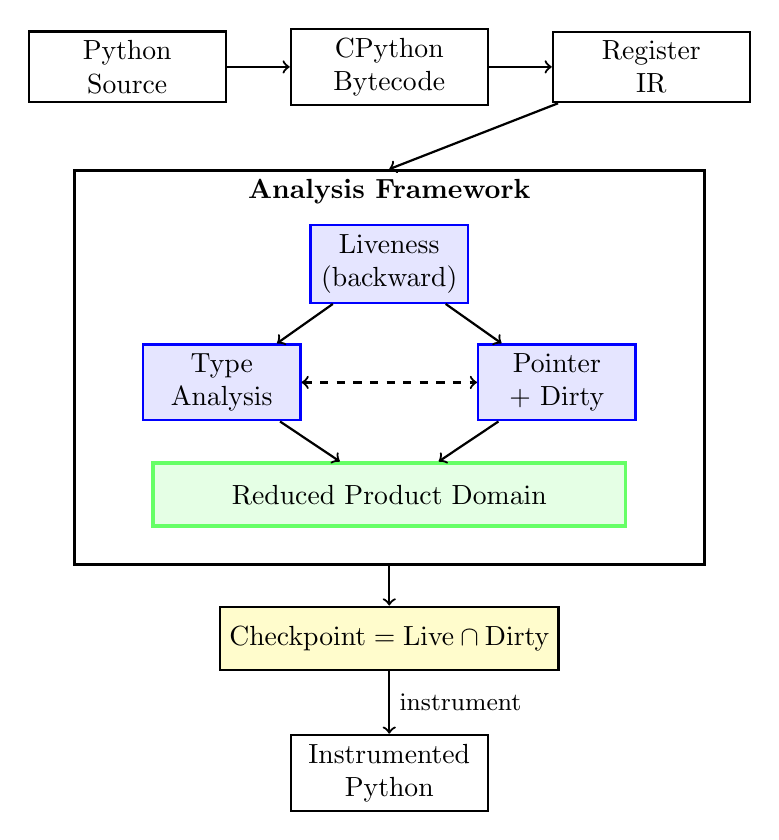
\begin{tikzpicture}[
    box/.style={rectangle, draw=black, thick, minimum width=2.5cm, minimum height=0.8cm, align=center},
    analysis/.style={rectangle, draw=blue, thick, minimum width=2cm, minimum height=0.6cm, align=center, fill=blue!10},
    arrow/.style={->, thick},
    darrow/.style={<->, thick, dashed},
    node distance=0.8cm
]

% Pipeline stages
\node[box] (source) {Python\\Source};
\node[box, right=of source] (bytecode) {CPython\\Bytecode};
\node[box, right=of bytecode] (ir) {Register\\IR};

% Analysis framework box
\node[rectangle, draw=black, very thick, minimum width=8cm, minimum height=5cm, below=0.8cm of bytecode] (framework) {};
\node[below] at (framework.north) {\textbf{Analysis Framework}};

% Three analyses inside framework
\node[analysis, below=1.5cm of bytecode] (liveness) {Liveness\\(backward)};
\node[analysis, below left=0.5cm and 0.1cm of liveness] (type) {Type\\Analysis};
\node[analysis, below right=0.5cm and 0.1cm of liveness] (pointer) {Pointer\\+ Dirty};

% Reduced product
\node[rectangle, draw=green!60, very thick, fill=green!10, minimum width=6cm, minimum height=0.8cm, below=2cm of liveness] (product) {Reduced Product Domain};

% Checkpoint equation
\node[box, fill=yellow!20, below=0.5cm of framework] (checkpoint) {$\text{Checkpoint} = \text{Live} \cap \text{Dirty}$};

% Instrumented code
\node[box, below=of checkpoint] (instrumented) {Instrumented\\Python};

% Arrows between pipeline stages
\draw[arrow] (source) -- node[right] {} (bytecode);
\draw[arrow] (bytecode) -- node[right] {} (ir);
\draw[arrow] (ir) -- (framework.north);
\draw[arrow] (framework.south) -- (checkpoint);
\draw[arrow] (checkpoint) -- node[right] {\small instrument} (instrumented);

% Arrows between analyses
\draw[arrow] (liveness) -- (type);
\draw[arrow] (liveness) -- (pointer);
\draw[darrow] (type) -- (pointer);
\draw[arrow] (type) -- (product);
\draw[arrow] (pointer) -- (product);

\end{tikzpicture}
\caption{Overview of our analysis pipeline. Python source is compiled to bytecode, translated to our register-based IR, then analyzed through three interacting analyses (liveness, type, and pointer+dirty tracking) combined in a reduced product domain. The intersection of live and dirty variables determines the minimal checkpoint set, which drives source-level instrumentation.}

    \caption{Analysis pipeline. Python source is compiled to bytecode, lowered to TAC, and analyzed in three interacting domains.}
    \label{fig:overview}
\end{figure}

\section{Analysis}
\label{sec:analysis}

Our static analysis framework combines several interacting domains to determine the minimal set of program variables that must be included in a checkpoint.  
We present the domains in an order that matches their conceptual dependencies, starting from the IR, then moving to liveness, explaining objects, and general domain conventions before introducing the specific domains for dirty tracking, pointers, and types. Figure~\ref{fig:overview} shows the full pipeline, from source code through IR, liveness, and the reduced product, to the extracted invariants used for checkpoint minimization.

\subsection{Intermediate Representation}
Our analyses operate not on Python source or bytecode directly, but on a simplified register-based \emph{three-address code} (TAC).
This IR is designed to make dataflow and heap accesses explicit, removing the operand stack of Python bytecode and any implicit temporaries.
A TAC program consists of a finite set of \emph{labels} $L$, each with an associated basic block of instructions.
Each instruction reads and writes explicit \emph{variables} $v \in \mathcal{V}$, which may be:
\begin{itemize}
    \item \emph{Named locals} (e.g.\ \texttt{x}, \texttt{result}), corresponding to function parameters and Python local variables.
    \item \emph{Stack variables} ($\$0, \$1, \ldots$), introduced during translation to replace Python's stack slots.
\end{itemize}
Control flow is represented explicitly in a \emph{control-flow graph} (CFG) $G = (L, E)$ with directed edges for possible execution paths.
We write $\mathsf{succ}(l)$ and $\mathsf{pred}(l)$ for the successors and predecessors of a label $l$ in $G$.
An \emph{instruction location} is denoted by $(l, i)$ for the $i$-th instruction in block $l$.
\subsection{Liveness Analysis}
Liveness analysis determines, for each program point, the set of TAC variables whose current value may be read along some future control-flow path before being overwritten.  
We compute liveness as a standard backward dataflow analysis on the TAC, with the set of live variables at a location $(l,i)$ denoted $\mathsf{Live}_{l,i} \subseteq \mathcal{V}$.

Related: \cite{pythonsemantics}.

\paragraph{Gen/Kill sets.}
For each instruction, we define:
\begin{itemize}
    \item $\mathsf{gen}$: the set of variables read by the instruction (whose current value is needed now).
    \item $\mathsf{kill}$: the set of variables definitely overwritten by the instruction (whose current value is no longer needed).
\end{itemize}
The backward transfer function is:
\[
\mathsf{Live}_{\mathrm{in}} = (\mathsf{Live}_{\mathrm{out}} \setminus \mathsf{kill}) \cup \mathsf{gen}.
\]
A variable in $\mathsf{kill}$ is said to be \emph{killed} at that instruction.

\paragraph{Variable kinds.}
Variables in $\mathcal{V}$ come in two forms:
\begin{itemize}
    \item \emph{Stack variables} ($\$0, \$1, \ldots$) are compiler-generated temporaries that exist only within a single basic block and cannot be addressed once they are dead.  
          Killing such a variable immediately removes any heap objects reachable from it from the root set.
    \item \emph{Named local variables} (e.g.\ \texttt{x}, \texttt{result}) persist for the duration of a function activation and may, in Python, be captured by closures or declared \texttt{nonlocal}.
          We restrict our target program subset to disallow such captures, so a named local can be considered dead when no further reads occur in the current function body.
\end{itemize}

\paragraph{Role in later domains.}
The live-variable set at each point is used to prune the root set for the pointer graph: when a variable $v$ is not live, all edges reachable only through $v$ are removed.
This prevents dead variables from keeping otherwise unreachable objects alive in the analysis state.

\subsection{Objects and Fields}
We model the heap as a finite set of \emph{abstract objects} $\mathcal{O}$, each representing either:
\begin{itemize}
    \item A distinguished \emph{root object} such as \texttt{LOCALS} or \texttt{GLOBALS}.
    \item A \emph{parameter object} representing a function argument at entry.
    \item An \emph{allocation site object} $o_{l,i}$ created by a specific instruction location $(l, i)$.
\end{itemize}
Objects have \emph{fields} $f \in \mathcal{F}$ representing attributes, dictionary keys, or sequence elements.
For collections, we use a wildcard field $\star$ to conservatively represent all indexed elements.
Accessing \texttt{x.f} refers to field $f$ of the object(s) currently bound to variable $x$.

We will write $P[o][f]$ for the set of target objects stored in field $f$ of object $o$ in the pointer graph (defined later), and $D[o]$ for the set of fields of $o$ that are currently dirty.

\subsection{Map Domains}
Many of our domains are \emph{maps}, i.e.\ finite partial functions $M : K \to V$ with a fixed \emph{default value} $\bot_V$ for missing keys.
We adopt a uniform notation and semantics for their use in abstract interpretation:
\begin{itemize}
    \item \textbf{Transfer:} An assignment to key $k$ replaces $M[k]$ with a new value $v$.
    \item \textbf{Weak update:} If $k$ may alias with other keys, we conservatively set $M[k] \leftarrow M[k] \sqcup v$ instead of overwriting.
    \item \textbf{Join:} $(M_1 \sqcup M_2)[k] = M_1[k] \sqcup M_2[k]$ for all $k$ in the union of their domains.
    \item \textbf{Subsumption:} $M_1 \sqsubseteq M_2$ if $M_1[k] \sqsubseteq M_2[k]$ for all $k$ in the union of their domains.
\end{itemize}
We treat missing keys as implicitly mapped to $\bot_V$ for the purposes of all operations above.
In our analyses, the value type $V$ may itself be another map, a set of objects, or a simple lattice such as booleans, making this pattern reusable across domains.

\subsection{Dirty Domain}
The \emph{dirty} domain maps each object to the set of fields written since the last checkpoint.
An update marks the corresponding field as dirty; deletions are treated as writes.
The domain itself does not decide which dirty objects must be checkpointed—this decision is deferred until pointer reachability and liveness are taken into account.
\subsection{Pointer Domain}
The \emph{pointer domain} models the shape of the heap as a map
\[
P : \mathcal{O} \to (\mathcal{F} \to \mathcal{P}(\mathcal{O}))
\]
where $P[o][f]$ is the set of abstract objects that may be stored in field $f$ of object $o$.
The inner map has default value $\emptyset$ for any field not explicitly present.

\paragraph{Transfer.}
On an instruction that stores a reference into a field---for example \texttt{x.f = y}---we first resolve the set of possible source objects $S$ for $y$ and the set of possible target objects $T$ for $x$.
For each $t \in T$, we update $P[t][f]$ with $S$.
If $t$ is known to be the only object bound to $x$ (no aliasing), we perform a \emph{strong update}:
\[
P[t][f] \leftarrow S.
\]
If aliasing is possible, we perform a \emph{weak update}:
\[
P[t][f] \leftarrow P[t][f] \cup S.
\]
Reads, such as \texttt{y = x.f}, do not change $P$ but are resolved by looking up $\bigcup_{t \in T} P[t][f]$.

\paragraph{Join and Subsumption.}
The join $P_1 \sqcup P_2$ is computed pointwise over objects and fields, taking the union of target sets.
Subsumption $P_1 \sqsubseteq P_2$ holds if $P_1[o][f] \subseteq P_2[o][f]$ for all $o \in \mathcal{O}$ and $f \in \mathcal{F}$.

\paragraph{Reachability.}
Given a set of \emph{root objects} $R \subseteq \mathcal{O}$ (typically \texttt{LOCALS} and \texttt{GLOBALS}), the set of \emph{reachable objects} $\mathsf{Reach}(R, P)$ is the smallest set containing $R$ and closed under:
\[
o \in \mathsf{Reach}(R, P) \wedge o' \in P[o][f] \implies o' \in \mathsf{Reach}(R, P).
\]
We use liveness to prune the roots $R$ before reachability is computed, ensuring that dead variables do not keep their objects alive.

\subsection{Type and Effect Domain}

Our type domain models Python values using a small set of constructs chosen to match the subset of Python we target: nominal classes, structural protocols, callable signatures, container types, and the special \texttt{any} type for unknown values.
Unlike general--purpose type systems, we unify the representation of parameter lists and object fields as \emph{rows}: finite ordered maps from keys (positional indices or names) to types.  
This gives a single mechanism for lookup, subtyping, joining, and unification across functions, classes, and modules.

Functions are annotated with \emph{effects} that describe their interactions with the heap: whether they allocate new objects, return existing ones, or update fields.  
These effects are directly consumed by the checkpointing analysis to determine which heap locations may be modified and which can be safely excluded from checkpoints.

\paragraph{Main type constructs.}
The principal forms in our type language (full syntax in Appendix~\ref{sec:appendix-typesystem}) are:
\begin{itemize}
  \item \textbf{Classes} $\mathsf{class}(C, R, \overline{\tau}, \overline{\alpha})$:
        a nominal class $C$ with row $R$ of fields and optional generic parameters $\overline{\alpha}$.
  \item \textbf{Protocols} $\mathsf{protocol}(R, \overline{\alpha})$:
        structural interfaces requiring the listed fields with given types, independent of nominal identity.
  \item \textbf{Modules}:
        rows of exported names and their types.
  \item \textbf{Functions} $\forall \overline{X}.\;R_{\mathrm{params}} \xrightarrow{\epsilon} \tau_{\mathrm{ret}}$:
        with parameter row $R_{\mathrm{params}}$, return type $\tau_{\mathrm{ret}}$, and effect $\epsilon$.
        Functions may appear in overload sets.
  \item \textbf{Other forms}:
        unions, generic instantiations, variadic packs for \texttt{*args}-style functions, and \texttt{any}.
\end{itemize}

\paragraph{Rows and subtyping.}
A row is a finite sequence of fields indexed by name or position.  
Width subtyping applies: a type with extra fields is a subtype of one with fewer fields, provided all shared fields match.  
Protocols are a special case: any object with the required fields is a subtype, regardless of its nominal class.

\paragraph{Call checking and binding.}
When a call is type--checked, argument types are unified with the corresponding parameter types:
\begin{itemize}
  \item Type variables may be solved, yielding a substitution applied to all remaining parameters and the return type.
  \item Parameters matched by the call are removed, producing either a \emph{residual callable} (for partial application) or the substituted return type.
  \item Variadic packs (\texttt{*args}) may be partially bound and matched incrementally; if unmatched packs remain, the result is again a residual callable.
\end{itemize}
Overloaded functions are handled by attempting binding against each arm independently; the results are joined when ambiguity remains.  
The formal residual--callable construction is given in Appendix~\ref{sec:appendix-typesystem}.

\paragraph{Effects.}
Effects annotate functions with heap interactions:
\begin{itemize}
  \item \textbf{\texttt{new}}: allocates a fresh object.
  \item \textbf{\texttt{points-to}}: returns a reference to an existing object.
  \item \textbf{\texttt{update}}: modifies or refines a specific field, possibly changing its type.
\end{itemize}
Updates are instantiated with actual arguments. For example, from the builtins stub:

\begin{lstlisting}[language=python]
@update(list[T | Q], 1)
def append[Q](self: list[T], x: Q) -> None: ...
\end{lstlisting}

If \texttt{self} initially has type \texttt{list[$\bot$]} and we call \texttt{append} with an \texttt{int}, the element type refines to \texttt{$\bot \sqcup$ list[$\bot$]} which is \texttt{list[int]}.  
Type-changing updates are only applied when the receiver is unaliased and monomorphic, preventing unsound refinements across aliases.

\paragraph{Field and attribute access.}
For $x.f$, the pointer domain yields possible receivers; their rows are inspected:
\begin{itemize}
  \item If all agree on the field type, that type is returned.
  \item If types disagree, their join is returned.
  \item If the field is missing, join with the residual row's default (often \texttt{any}) and mark as possibly failing.
\end{itemize}

\paragraph{Example: partial application and update.}
Consider:
\[
f : \forall T,U.\; (0:T, 1:U) \to T
\]
Calling $f$ with an \texttt{int} yields a residual $(0:U) \to \texttt{int}$.  
Calling this residual with a \texttt{str} then yields a residual  $() \to \texttt{int}$; finally, retrieving the result yields an \texttt{int}.  
Similarly, \texttt{list.append} with an \texttt{int} argument refines the element type from unknown to \texttt{int}.

\paragraph{Precision and limits.}
The type system can:
\begin{enumerate}
  \item Identify exactly which heap locations an operation may modify.
  \item Exclude immutable structures from checkpoints.
  \item Refine container element types across updates.
\end{enumerate}
Precision loss occurs when joins force widening to \texttt{any} (e.g., differing field types, many unknowns, or unknown attribute names).  
Dynamic features such as monkey--patching, dynamic imports, or metaclass manipulation are excluded from the target subset.

\subsection{Domain Interactions}
The domains operate in a reduced product with directed information flow:
\begin{itemize}
    \item \emph{Liveness $\rightarrow$ Pointer:} prunes unreachable roots and their edges.
    \item \emph{Type $\rightarrow$ Pointer:} constrains possible targets based on type-level field shape.
    \item \emph{Type $\rightarrow$ Dirty:} immutable objects never become dirty.
    \item \emph{Pointer $\rightarrow$ Type:} dynamic dispatch resolution is narrowed to types of reachable receivers.
\end{itemize}
These interactions improve precision by removing impossible states before they can pollute other domains.

\subsection{Transfer Functions}
For each TAC instruction, the transfer function updates only the affected keys in each domain according to the instruction’s semantics.
Weak updates are applied when aliasing is possible, and joins are used when merging control-flow paths.
The set of checkpoint roots at loop boundaries is obtained by intersecting live roots with reachable dirty objects.



\begin{table}
\centering
\begin{tabular}{l|r|r|r|r}
\toprule
\textbf{Benchmark} & 
\multicolumn{1}{c}{\textbf{\spyte}} &
\multicolumn{1}{c}{\textbf{Locals}} &
\multicolumn{1}{c}{\textbf{\PROCDIFF}} &
\multicolumn{1}{c}{\textbf{\VMDIFF}} \\
\midrule
\multirow{2}{*}{\texttt{noploop}} & 72 & 75 & \textbf{14} & 17966 \\
 &  & {\footnotesize 1.04$\times$} & {\footnotesize 0.19$\times$} & {\footnotesize 249.52$\times$} \\
\midrule
\multirow{2}{*}{\texttt{pivoter}} & \textbf{226} & 261 & 516 & 23400 \\
 &  & {\footnotesize 1.15$\times$} & {\footnotesize 2.28$\times$} & {\footnotesize 103.48$\times$} \\
\midrule
\multirow{2}{*}{\texttt{kmeans}} & \textbf{270} & 9136 & 51418 & 254554 \\
 &  & {\footnotesize 33.84$\times$} & {\footnotesize 190.44$\times$} & {\footnotesize 942.79$\times$} \\
\midrule
\multirow{2}{*}{\texttt{omp}} & \textbf{3593} & 457358 & 832266 & 130034290 \\
 &  & {\footnotesize 127.29$\times$} & {\footnotesize 231.64$\times$} & {\footnotesize 36191.01$\times$} \\
\bottomrule
\end{tabular}
\caption{Average checkpoint sizes (in bytes) across filtered iterations. Small text shows size relative to \spyte.} \centering
\label{tab:checkpoint-sizes}
\end{table}

\section{Evaluation}
\label{sec:evaluation}
We evaluate our approach to program-guided checkpointing on four Python workloads: \texttt{noploop}, \texttt{pivoter}, \texttt{kmeans}, and \texttt{omp}. These benchmarks capture common iterative patterns in numerical computing and machine learning, with varying degrees of control complexity, memory reuse, and heap allocation behavior. In each, we insert checkpoint instrumentation at the head of the primary loop, allowing recovery from the beginning of any iteration. We measure the size of the persisted state after each checkpoint operation.

\begin{itemize}[leftmargin=*]
    \item \textbf{noploop} is a degenerate  {\color{blue!50!black}
\texttt{for}~\textrm{...}~\texttt{in}~\texttt{range}} loop with no meaningful computation or allocation except the iterator. It serves as a lower bound on checkpointing overhead. We run the loop for 100 steps.

    \item \textbf{pivoter} (26 LOC, 2 out of 7 relevant variables) performs clique enumeration over a sparse graph via depth-first search and backtracking~\cite{jain2020power}. Program state is encoded in sets and counters. Input is a 100-node, 757-edge subgraph extracted from the Enron dataset. The algorithm requires $\sim 47,000$ steps to complete. Due to the computational cost of process- and VM-level checkpointing, we sample checkpoints every 50 or 51 steps (yielding 1,891 checkpoint pairs total), but measure memory differences between consecutive snapshots to estimate per-step deltas. This avoids the cost of capturing all 47,000 steps while maintaining fair comparison granularity.

    \item \textbf{kmeans} (15 LOC, 1 out of 10 relevant variables) implements K-Means clustering on synthetic data~\cite{macqueen1967multivariate}. Each iteration reassigns samples to centroids and updates them. Only the centroid array needs to persist. Data is generated using \texttt{sklearn.datasets.make\_blobs} with $\textit{n\_samples}=1000$, $\textit{n\_features}=2$, $k=5$. The algorithm completes in 20 steps.

    \item \textbf{omp} (42 LOC, 2 out of 21 relevant variables)---Orthogonal Matching Pursuit is a greedy feature selection algorithm~\cite{Pati1993OMP, quinzan2022fast}. At each step, it selects the feature most correlated with the residual and retrains a regression model from scratch. The input is the \texttt{healthstudy} dataset with $k = 35$. The algorithm completes in 35 steps.
\end{itemize}

All benchmarks use fixed data and identical loop structure across checkpointing configurations. Dataset selection was finalized before implementing or evaluating instrumentation.

\begin{itemize}[leftmargin=*]
  \item \textbf{Locals}: Pickling (Python data serialization) all local variables (excluding parameters), regardless of whether they were modified or needed again.
  \item \textbf{\PROCDIFF}: We implemented process-level checkpointing using a custom tool that captures all writable memory regions by reading from \texttt{/proc/self/mem}. We initially attempted to use CRIU for process-level checkpointing, but found its memory overhead dominated the storage costs by orders of magnitude, making meaningful comparison impractical. 
  \item \textbf{\VMDIFF}: VM-level checkpointing based on snapshots and 64-byte memory diffing between iterations. The checkpoints are taken by triggering QEMU memory dumps via QMP commands over TCP.
\end{itemize}

We omit the first iteration of each benchmark (since no diff can be computed). We also omit the final two iterations, which introduce irregularities in the {\PROCDIFF} and {\VMDIFF} baselines.

\paragraph{Notes on Overhead Accounting}
The use of TCP to trigger VM-level checkpoints may introduce a nontrivial fixed overhead per snapshot. While difficult to isolate, we partially control for such effects by comparing deltas between consecutive snapshots rather than absolute snapshot sizes. In contrast, \spyte and {Locals} Python checkpoints use direct pickle serialization. Thus, while our VM-level measurements reflect realistic system-level behavior, they may slightly overestimate true memory diffs compared to language-level checkpointing.

\begin{figure*}[t]
    \centering
  \ifdraft[redacted by \texttt{ifdraft}]\else
    % \tikzset{external/force remake}

% \PlotExp{<Title>}{<CSV path>}{<Prefix>}
\newcommand{\PlotExp}[3]{%
  % \DependOnCSV{#2}% ensures rebuild if the CSV changes
  \nextgroupplot[title={#1}]
  \pgfplotstableread[col sep=comma,trim cells]{#2}\datatable

  % Per-row bands for proc0..4
  \pgfplotstablecreatecol[
    create col/expr={min(min(min(min(\thisrow{proc0},\thisrow{proc1}),\thisrow{proc2}),\thisrow{proc3}),\thisrow{proc4})}
  ]{procmin}{\datatable}
  \pgfplotstablecreatecol[
    create col/expr={max(max(max(max(\thisrow{proc0},\thisrow{proc1}),\thisrow{proc2}),\thisrow{proc3}),\thisrow{proc4})}
  ]{procmax}{\datatable}

  % Per-row bands for vm0..4
  \pgfplotstablecreatecol[
    create col/expr={min(min(min(min(\thisrow{vm0},\thisrow{vm1}),\thisrow{vm2}),\thisrow{vm3}),\thisrow{vm4})}
  ]{vmmin}{\datatable}
  \pgfplotstablecreatecol[
    create col/expr={max(max(max(max(\thisrow{vm0},\thisrow{vm1}),\thisrow{vm2}),\thisrow{vm3}),\thisrow{vm4})}
  ]{vmmax}{\datatable}

  % Bands (unique name paths via prefix #3)
  \addplot[name path=#3PROCmax, draw=none] table[x=i, y=procmax]{\datatable};
  \addplot[name path=#3PROCmin, draw=none] table[x=i, y=procmin]{\datatable};
  \addplot[fill opacity=0.14, draw=none] fill between[of=#3PROCmax and #3PROCmin];

  \addplot[name path=#3VMmax, draw=none] table[x=i, y=vmmax]{\datatable};
  \addplot[name path=#3VMmin, draw=none] table[x=i, y=vmmin]{\datatable};
  \addplot[fill opacity=0.14, draw=none] fill between[of=#3VMmax and #3VMmin];

  % Central lines
  \addplot[very thick] table[x=i, y=procavg]{\datatable};
  \addplot[very thick, dashed] table[x=i, y=vmavg]{\datatable};
  
    \addplot[
      only marks,
      mark=diamond*,
      mark options={blue}
    ] table[x=i, y=naive]{\datatable};
    
    \addplot[
      only marks,
      mark=asterisk,
      mark options={red}
    ] table[x=i, y=instrumented]{\datatable};
}

% \tikzsetnextfilename{benchmarks-fourpanel} % cache file: tikz-cache/benchmarks-fourpanel.pdf
\begin{tikzpicture}
\begin{groupplot}[
    group style={
        group size=2 by 2,
        horizontal sep=2cm,
        vertical sep=2cm
    },
    width=0.48\textwidth,
    height=0.35\textwidth,
    xlabel={$i$},
    ylabel={Bytes},
    ymode=log,
    xtick=\empty,
    xticklabel=\pgfmathprintnumber{\tick},
    xtick distance=1,
    % ymin=9,
    % ymax=3e8,
    grid=major,
    title style={yshift=-1ex},
    legend to name=grouplegend,
    legend columns=4,
    legend style={/tikz/every even column/.append style={column sep=1em}, draw=none, font=\small, anchor=north}
]

\PlotExp{\texttt{noploop}}{experiments/noploop.csv}{A}
\PlotExp{\texttt{pivoter}}{experiments/pivoter.csv}{B}
\PlotExp{\texttt{kmeans}}{experiments/kmeans.csv}{C}
\PlotExp{\texttt{omp}}{experiments/omp.csv}{D}

\end{groupplot}

\end{tikzpicture}
\vspace{1ex} % optional spacing
\begin{center}


\pgfplotslegendfromname{grouplegend}
% Define legend items here (OUTSIDE the plot):
\begin{tikzpicture}
  \begin{axis}[
      hide axis,
      scale only axis,
      xmin=0, xmax=1, ymin=0, ymax=1, % force non-empty range
      legend columns=3,
      legend style={draw=none, /tikz/every even column/.append style={column sep=1em}}
    ]

    \addlegendimage{area legend, fill=black!15, draw=none}
    \addlegendentry{\VMDIFF\;min--max band}

    \addlegendimage{area legend, fill=gray!30, draw=none}
    \addlegendentry{\PROCDIFF\;min--max band}

    \addlegendimage{only marks, mark=diamond*, mark options={blue}}
    \addlegendentry{Naive}
    
    \addlegendimage{line legend, black, dashed}
    \addlegendentry{\VMDIFF\;Average}

    \addlegendimage{line legend, black}
    \addlegendentry{\PROCDIFF\;Average}

    \addlegendimage{only marks, mark=asterisk, mark options={red}}
    \addlegendentry{Instrumented}

  \end{axis}
\end{tikzpicture}
\end{center}
\caption{Memory usage per checkpointing method across four benchmarked programs}

  \fi
  \caption{Memory snapshot sizes across iterations for four benchmarks, comparing process-level, VM-level checkpointing with application-level methods: keeping all local variables, and our method \spyte. Lines show averages over five runs; shaded bands indicate min-max ranges across runs. Y-axis is logarithmic. In \texttt{noploop} (top-left), {Locals} and \spyte values overlap.}
  \label{fig:snapshot-graph}
\end{figure*}

\subsection{Checkpoint Size Comparison} 
\Cref{tab:checkpoint-sizes} reports the mean size in bytes of each checkpointing method after filtering. Our system consistently outperforms both Local variables checkpointing and simulated Process- and VM-level methods. ``\spyte'' refers to the instrumented version produced by our static analysis-based checkpointing. ``\PROCDIFF'' and ``\VMDIFF'' refer to memory differentials at the process and virtual machine levels respectively.

For the \texttt{noploop} benchmark, our analysis incurs a fixed overhead (iterator) that exceeds 
the minimal state changes, making process-level diffing more efficient. This represents a limitation for programs with very small persistent state.

The \texttt{pivoter} benchmark, a recursive clique enumeration program, maintains small internal state (e.g., recursion depth and adjacency buffers) that is genuinely required to resume computation. Our system’s performance is nearly identical to the process-level memory diff, suggesting that it is near-optimal in this case; in contrast, naively checkpointing all local variables leads to 10x memory overhead. The \texttt{noploop} benchmark confirms the lower bound: our instrumentation adds minor overhead (e.g., iterator state), while process-level diffing captures the true minimal footprint. Comparing \PROCDIFF results between \texttt{pivoter} and \texttt{noploop} reveals that process snapshots can be highly efficient in simple cases, adding as little as 23 bytes of overhead.

In \texttt{kmeans}, \spyte achieves significant reductions: $33.84\times$ smaller than {Locals}, $190.44\times$ smaller than \PROCDIFF, and $942.79\times$ smaller than \VMDIFF. This improvement stems from excluding transient arrays---gradients, distances, and cluster metrics---that are allocated per iteration and dead by the loop's end. The \texttt{omp} benchmark shows even more dramatic gains ($127.29\times$, $231.64\times$, and $36191.01\times$ smaller, respectively) because its large working arrays and regression buffers are reused rather than persisted, allowing our dirty-pointer analysis to exclude them from checkpoints.

Beyond these average sizes, examining checkpoint behavior across iterations reveals interesting temporal patterns. \Cref{fig:snapshot-graph} visualizes the per-iteration checkpoint sizes for each technique across our four benchmarks. The plots reveal distinct patterns in checkpoint behavior. In \texttt{noploop}, \PROCDIFF maintains minimal state except for a notable spike mid-execution (likely from buffer reallocation) while our method tracks closely with {Locals} (showing pure checkpoint overhead).
The \texttt{pivoter} benchmark, with its many iterations, shows periodic bursts in checkpoint sizes across all methods; however, \spyte exhibits notably more stable behavior with less dramatic spikes compared to both {Locals} and \PROCDIFF. This stability is advantageous for network transmission and storage systems where sudden bursts can cause latency issues. Note that each point is a diff of two consecutive iterations, not over the 50-step jumps.
The \texttt{kmeans} benchmark demonstrates relatively constant checkpoint sizes across iterations for all techniques, with our method maintaining significant size advantage consistently throughout execution. Notably, \texttt{omp} reveals a critical scaling difference: while most methods show steadily increasing checkpoint sizes as iterations progress (with slopes greater than 1), \spyte maintains a much gentler slope, meaning our performance advantage actually increases with longer-running computations. Across all benchmarks, \VMDIFF exhibits higher variance between runs (visible in the wider shaded bands), while other techniques show more consistent behavior across different executions, with application-level methods (\spyte and {Locals}) having zero variance. These patterns confirm that our static analysis not only reduces average checkpoint size but also provides more predictable and stable checkpointing behavior.

Overall, our results show that the combination of static analysis and lightweight dynamic instrumentation can exclude large volumes of memory that are either unmodified or recomputable, particularly in numerical programs with regular iterative structure.

\subsection{Discussion}

The results support the following observations:

\begin{itemize}
  \item \textbf{Static analysis can yield substantial reductions} in checkpoint size when recomputation is cheap and allocation is disciplined. This aligns with common usage patterns in numerical and data science code.
  \item \textbf{VM- and Process-level diffs greatly overapproximate state necessity}: they include any dirty memory, even if transient or unused, leading to high checkpoint costs.
  \item \textbf{Analysis precision is workload-sensitive}: the benefits are most pronounced when mutable state is well-localized, heap aliasing is limited, and control structure is predictable.
  \item \textbf{Application-level checkpointing improves predictability}: The \spyte method shows more stable checkpoint sizes across runs, with minimal variance and gentler growth rates across iterations compared to system-level approaches.
\end{itemize}

\subsection{Limitations and Threats to Validity}
\label{sec:threats}

Our system assumes that all side effects are either annotated or internal to the function body. If external state is dirty (e.g., global variables, files, sockets) and not captured by the type system, recovery may be unsound.

Additionally, our analysis does not verify behavioral equivalence post-recovery. We produce an explicitly instrumented version of the code so programmers can double-check it themselves. We rely on programmer discipline and the assumption that the relevant control path is idempotent from the checkpoint location onward.

Our analysis takes a few seconds per benchmark function, and can be run entirely ahead-of-time. This is fast enough to be usable in practice and supports iterative development. We do not report fine-grained performance numbers, as the tool is not designed to operate online or scale to large codebases; rather, its value lies in enabling precise transformations in tightly scoped, performance-critical numerical kernels.

\section{Related Work}
\label{sec:related}

\subsection{Static Analysis of Dynamically-Typed Languages}
Static analysis of dynamically typed languages presents a unique challenge due to their lack of explicit type annotations, dynamic object structures, and runtime features such as \texttt{eval} and dynamic attribute creation. A significant body of research has addressed these challenges, with approaches ranging from type inference and alias analysis to abstract interpretation over rich semantic domains.

\paragraph{Type and Pointer Analysis in Python.}
Early efforts at type analysis for Python include Starkiller~\cite{salib2004starkiller}, a whole-program ahead-of-time compiler performing interprocedural type inference. Starkiller demonstrated the feasibility of static compilation for a large subset of Python by modeling control-flow and using a variant of the Cartesian Product Algorithm. RPython~\cite{ancona2007rpython} took a more restrictive route, defining a statically analyzable subset of Python suitable for ahead-of-time translation, forming the basis of the PyPy project.

Subsequent work focused on formalizing type analysis through abstract interpretation. Fritz and Hage~\cite{fritz2017cost} evaluated configurable approximate typing for Python, showing that flow-insensitive treatment of module-scope variables improves both speed and precision, while call-site sensitivity adds cost with little precision benefit.
More recently, Fromherz et al.~\cite{fromherz2018static} and Monat et al.~\cite{monat2021static}~\cite{monat2021multilanguage} developed abstract interpreters over custom domains capable of analyzing control-flow-sensitive types and values, including object-oriented features, exceptions, and generators. The latter system, \textbf{Mopsa}, models both nominal and structural typing, deals with C extensions, and tracks container shapes and type equality relationships. In its pointer analysis, Mopsa uses \emph{recency abstraction}, keeping the most recent pointer value in addition to the combined value for other iterations, which enhances precision. We've found no need for this abstraction in the programs we analyzed. 

Beyond specific analyses, Li et al.\ introduced Scalpel~\cite{li2022scalpel}, a general-purpose static analysis framework for Python.

Aliasing in Python---analogous to pointer analysis---has also been studied. Gorbovitski et al.~\cite{gorbovitski2010alias} proposed a flow- and context-sensitive alias analysis for Python, enabling optimizations like memoization.

\paragraph{Practical Tools for Python.}
Gradual type checkers such as Mypy~\cite{mypy}, Pyre~\cite{pyre}, and Pytype~\cite{pytype} are widely used in practice. While unsound by design, they use flow-sensitive and partially context-sensitive type inference to catch common bugs and enable scalable static typing. Pytype notably employs abstract interpretation internally, treating variables and control-flow through a form of symbolic execution over types and heap aliases. These tools sacrifice soundness for usability, offering fast feedback and integration with developer workflows.

\paragraph{Abstract Interpretation in Other Dynamic Languages.}
The use of abstract interpretation is well-established in the analysis of other dynamic languages. For JavaScript, TAJS~\cite{jensen2009type} and JSAI~\cite{kashyap2014jsai} applied abstract interpretation to model ECMAScript features such as prototype inheritance and dynamic property creation. JSAI's design incorporates a reduced product of domains for type, pointer, numeric, and string analysis. These frameworks support sound over-approximations of JavaScript semantics and demonstrate high configurability and modularity.

In Ruby, the DRuby system~\cite{furr2009static} introduced a sophisticated type language with union and intersection types, modeling Ruby's dynamic method dispatch. RDL and InferDL~\cite{kazerounian2020sound} extend this work by inferring and refining types using heuristics and partial static analysis. SimTyper~\cite{kazerounian2021simtyper} proposes sound type inference for Ruby by combining constraint-based inference with machine learning-based type equality prediction. Using a neural similarity model (DeepSim), SimTyper refines overly general types to more usable ones, matching programmer-written annotations while preserving soundness.

Lua also saw the introduction of Typed Lua~\cite{maidl2014typed}, which defines a gradual type system with union types and subtyping. Practical variants like Luau (Roblox) and Teal build on these ideas to enable static checking in large-scale Lua applications.

\paragraph{Static Analysis for Compilation and Specialization.}
A major motivation for static analysis of dynamic languages has historically been ahead-of-time compilation and runtime specialization. Starkiller~\cite{salib2004starkiller} targeted static compilation, while RPython~\cite{ancona2007rpython} defines a restricted, analyzable subset of Python enabling C code generation and tracing JITs in PyPy. In JavaScript, systems like TAJS~\cite{jensen2009type} and JSAI~\cite{kashyap2014jsai} support aggressive optimization and specialization. Related strategies have been adopted in Ruby and Lua to enable efficient execution or compilation. Even in more static languages like Julia, type inference underpins aggressive method specialization and inlining. Across these efforts, the analysis result is consumed to produce faster code --- either at compile time or as part of a just-in-time execution strategy.

\paragraph{Static Analysis for Program Transformation.}
Beyond compilation, static analysis has occasionally been used to guide automated transformations for purposes other than performance. Gorbovitski et al.~\cite{gorbovitski2010alias} use alias analysis in Python to enable automatic memoization of function calls. In JavaScript, abstract interpretation has been used to generate instrumentation for profiling and taint tracking. These works exemplify a broader but less explored class of applications in which analysis drives transformation, modifying the program or its runtime behavior based on inferred properties. Our work falls into this category, but targets a distinct goal: using type and pointer information to automatically manage and prune checkpoints in Python programs. To our knowledge, this is the first application of static analysis for dynamic languages aimed at improving recoverability through transformation of the program’s state management.

\subsection{Static Analysis-Based Checkpointing}

Static analysis has long been used to optimize checkpointing by identifying which portions of program state are necessary for correct recovery. Early work such as CATCH by Li and Fuchs~\cite{li1990catch} demonstrated the feasibility of using compiler-based liveness analysis and memory classification to exclude dead or recomputable data from checkpoints in Fortran and C programs. While foundational, this work was limited to relatively rigid memory models.

Rodríguez et al.~\cite{rodriguez2010cppc} developed CPPC, a source-to-source compiler for MPI applications that applies interprocedural data-flow analysis to automatically insert variable-level checkpoints. The static analysis component is essential in abstracting over low-level, non-portable state and allowing transparent instrumentation, particularly in distributed environments.

Vogt et al.~\cite{vogt2015lightweight} extend LLVM to support high-frequency user-level checkpointing via byte-level memory instrumentation. While their work focuses on runtime performance, it crucially relies on LLVM's data structure analysis (a context- and field-sensitive points-to analysis) to identify non-escaping memory objects --- a form of checkpoint escape analysis --- which are then excluded from instrumentation. This use of static pointer analysis improves performance by reducing unnecessary state tracking, particularly for stack and transient heap data.

Kim et al.~\cite{kim2024lact} apply array-level liveness analysis to reduce checkpoint overhead in intermittent computing environments. Their approach statically analyzes memory access patterns across loop structures to determine which portions of arrays are no longer live at checkpoint sites. This static pruning substantially reduces energy and storage costs in sensor workloads where large arrays dominate memory usage.

De Kruijf et al.~\cite{de2012static} propose \textit{idempotent processing}, a compiler-based technique that partitions programs into statically identified re-executable regions. These regions are guaranteed to produce the same results on re-execution, allowing recovery without checkpointing. Their work uses control- and data-flow analysis to identify safe region boundaries and optimize speculative execution without requiring hardware rollback.

\section{Conclusion}
We have presented a static analysis framework tailored to a practical subset of Python, enabling precise liveness, type, and pointer analyses to identify the minimal set of variables that must be preserved across checkpoints in iterative programs. By combining these analyses in a reduced product domain, our approach significantly reduces checkpoint size without sacrificing correctness, even in a highly dynamic language. Experiments on realistic workloads demonstrate that this method achieves substantial memory savings with negligible runtime overhead. Beyond checkpointing, the framework offers a foundation for other transformations that require fine-grained reasoning about program state in Python.

\appendix
\appendix
\section{Analysis Assumptions and Design Trade-offs}
\label{sec:appendix-assumptions}

To ensure a sound and tractable static analysis of a highly dynamic language, our framework targets a well-defined and practical subset of Python programs. This section outlines the scope of our analysis and the key design trade-offs that balance implementation complexity with analytical precision.

\paragraph{Target Program Scope}
Our analysis requires that programs adhere to the following properties, which enable a sound interpretation of control and data flow:
\begin{itemize}
    \item \textbf{No Dynamic Code Evaluation:} Constructs such as \texttt{eval}, \texttt{exec}, and \texttt{getattr} with dynamically computed string arguments are disallowed. These features prevent the static resolution of the program's control-flow graph.
    \item \textbf{Statically-Resolvable Calls:} Function calls must be resolvable at analysis time using the provided type signatures. The framework does not model complex higher-order control flow where functions are passed as first-class values to unknown call sites.
    \item \textbf{Explicit Generic Instantiations:} To avoid relying on runtime type propagation, generic collections must be explicitly instantiated with their type parameters (e.g., \texttt{list[int]()}), especially when empty.
    \item \textbf{Simplified NumPy Aliasing:} The analysis assumes that NumPy array variables refer to distinct memory objects unless explicitly constructed via view-creating operations. It does not model view-based aliasing where multiple arrays may share the same underlying data buffer.
\end{itemize}

These assumptions are satisfied by a wide class of numerical programs that follow idiomatic NumPy usage: preallocated buffers, explicit data copying, no implicit sharing, and simple iteration over typed arrays. These assumptions enable a sound, precise static analysis tailored to checkpointing in deterministic, structured Python programs.

\paragraph{Precision and Design Trade-offs}
Within this scope, our analysis embodies several conscious design trade-offs. Some choices simplify the abstract domain at the cost of precision, while others introduce complexity to the type system to more faithfully model Python's idioms and avoid hardcoding.
\begin{itemize}
    \item \textbf{Dimensionality-Agnostic Array Types:} The type system abstracts all \texttt{numpy.ndarray} objects as containing floating-point numbers but does not track their dimensionality or shape. This design greatly simplifies the typing of numerical operations but means the analysis cannot distinguish between a vector and a matrix, which in some cases may require additional user hints to ensure type precision.
    \item \textbf{Wildcard for Collection Elements:} To handle collections of arbitrary size and for accesses that are not precisely known, our pointer analysis models all element access (e.g., via subscripting) using a single wildcard field, \texttt{*}. This is efficient and scalable but merges the abstract state of all elements, meaning a write to one index will appear to affect all others.
    \item \textbf{Literal Types for Precision:} We chose to add complexity by incorporating literal types (e.g., \texttt{Literal["mean"]}) into the type system. While this makes the type hierarchy more complex, it enables a fully generic, type-driven model for attribute access. It allows the analysis to resolve expressions like \texttt{x.mean} by treating it as a subscription on \texttt{x}'s type with the literal value, avoiding hardcoded heuristics for method names.
    \item \textbf{Variadic Generics for Generality:} The type system supports variadic generics (e.g., \texttt{*Args}). This required a more complex unification algorithm but was useful to accurately model common Python constructors like \texttt{tuple()} without special-casing them in the analyzer. This design allows the framework to be more extensible and handle a wider range of idiomatic Python code in a principled way.
    \item \textbf{Reliance on Annotations:} The soundness of the analysis is contingent on the correctness and completeness of the provided type and side-effect annotations (e.g., \texttt{new}, \texttt{update}). This is particularly true for external library functions, which are modeled as black boxes whose behavior is determined entirely by these summaries. Verifying these annotations is currently a manual process.
\end{itemize}


\newpage

\section{TAC Intermediate Representation}
\label{sec:appendix-tac-ir}

\subsection{Overview and Motivation}

Static analyses typically operate over intermediate representations (IRs) rather than source code or execution format. IRs provide a compact and regularized view of programs that eliminates language-specific details, makes implicit temporaries explicit, and exposes dataflow for uniform analysis.

In our setting, we target Python programs as executed by \emph{CPython}, the reference implementation.  
CPython compiles source into a stack-based bytecode, designed primarily for interpreter simplicity, portability, compact code generation and efficient execution. 
While these properties make CPython bytecode effective as an execution format, they make it poorly suited to static reasoning: analysis would be entangled with stack shuffling and other incidental execution mechanics.

We therefore compile CPython bytecode into a dedicated verification-oriented IR, which we call \emph{Three-Address Code (TAC)}.  
TAC is register-like: every intermediate value is explicitly named, and heap operations (field access, subscripting, calls) are represented uniformly.  
TAC is not a new execution format, but an analysis-oriented abstraction that cleanly separates semantic operations from stack mechanics.

This IR serves three purposes for our checkpointing analysis:
\begin{enumerate}
    \item \textbf{Explicit data flow.} Variable reads and writes are fully explicit, enabling precise liveness analysis.
    \item \textbf{Uniform heap modeling.} Attributes, subscripts, and calls are normalized, simplifying pointer and alias reasoning.
    \item \textbf{Stable substrate for inference.} With stack effects eliminated, type and effect inference can operate directly on visible dependencies.
\end{enumerate}

TAC is the common foundation for the liveness, pointer, and type domains that drive our checkpointing optimization framework (\autoref{sec:analysis}, \autoref{sec:appendix-typesystem}).

In this appendix we present the syntax and operational semantics of TAC, followed by its translation from CPython bytecode.  
We conclude with key properties of the IR and a discussion of design choices and limitations.


\begin{figure}[t]
\centering
\[
\begin{aligned}
\textbf{Instructions:} && \\
cmd ::= \;& \mathsf{Assign}(\sigma, e) \\
      &\mid \mathsf{Assume}(\$b, true|false) \\
      &\mid \mathsf{For}(\$n, \$s_{\mathit{iter}}, \ell_{\mathit{exit}}) \\
      &\mid \mathsf{Exit} \\[1ex]
\textbf{Expressions:} && \\
e ::= \;& s \mid v \mid c \\
 &\mid \mathsf{Attribute}(s, f) \\
 &\mid \mathsf{Subscript}(s_1, s_k) \\
 &\mid \mathsf{Binary}(op, s_1, s_2, inplace) \\
 &\mid \mathsf{Unary}(op, s) \\
 &\mid \mathsf{Call}(s_f, \overline{s}, \ell) \\[1ex]
\textbf{Assignment Targets:} && \\
s ::= \;& \mathsf{\$}i \\
\sigma ::= \;& id \mid \mathsf{Attribute}(s,f) \mid \mathsf{Subscript}(s_1,s_2) \mid \langle\overline{s}\rangle
\end{aligned}
\]
\caption{TAC Syntax}
\label{fig:tac-syntax}
\end{figure}

\subsection{Programs and Control Flow}

A TAC program is represented as a control-flow graph that makes execution paths explicit for dataflow analysis. This representation directly supports our liveness analysis (which requires predecessor/successor relationships) and loop-aware checkpointing (which needs to identify iteration boundaries).
A program is a control-flow graph whose edges are annotated with TAC instructions.
Basic blocks contain straight-line instruction sequences with no internal control flow. Control transfers occur only at block boundaries via explicit edges in the graph. This structure enables efficient dataflow analysis by providing clear program points where analysis state must be merged or propagated.
Raising exceptions is allowed, but handling them is not; \texttt{raise} is handled as a terminating instruction. \texttt{yield} is unsupported. Both decisions prevent the control flow from becoming unmanageable. 

\subsection{Syntax}

\paragraph{Meta-Notation.}
In the formal definitions that follow, sequences are written with overlines and bounds (e.g.\ $\overline{x}_{i=1}^{n}$ where $n \geq 0$).

\paragraph{Instructions.}
Instructions in TAC represent the atomic units of computation and control flow.
Each instruction corresponds to a single semantic action in Python but is normalized
to eliminate incidental stack mechanics. This makes dataflow explicit and simplifies
analysis. The instruction set includes:
\begin{itemize}
    \item \textbf{\textsf{Assign}$(\sigma, e)$}: Evaluates expression $e$ and writes the result to target $\sigma$. Targets may include tuple unpacking and attribute/subscript assignments.~\footnote{The implementation also handles CPython's \texttt{LOAD\_FAST\_AND\_CLEAR} opcode, used in comprehensions to prevent variable capture, using a flag to handle push-pop of a potentially nonexistent named variable. We omit this detail in the formal description for simplicity.}
    \item \textbf{\textsf{Assume}$(\$b, true)$}: continues execution iff $\$b$ is exactly the object corresponding to Python's \texttt{True} (and similarly \textsf{Assume}$(\$b, false)$).
    \item \textbf{\textsf{For}$(\sigma, v_{\mathit{iter}}, \ell_{\mathit{exit}})$}: Implements a Python \texttt{for} loop by binding each value from the iterator $v_{\mathit{iter}}$ to target $\sigma$. Control jumps to $\ell_{\mathit{exit}}$ when the iterator is exhausted.
    \item \textbf{\textsf{Exit}}: Terminates the current control-flow path (function return or raising an exception).
\end{itemize}

Key design elements include:
\begin{itemize}
    \item \textbf{Assignment targets} $\sigma$ support Python's flexible assignment patterns, including tuple unpacking and attribute/subscript assignment.
    \item \textbf{Expressions} $e$ cover all Python operations needed for numerical code: arithmetic, attribute access, subscripting, and function calls.
    \item \textbf{Control flow} is statically known via graph edges.
\end{itemize}

\paragraph{Expressions.}
Expressions in TAC are designed to make all data dependencies explicit. Variables $v$ and constants $c$ form the atomic expressions, while compound expressions (\textsf{Attribute}, \textsf{Subscript}, \textsf{Binary}, \textsf{Unary}, \textsf{Call}) represent Python's primary operations. The \textsf{Binary} expression includes an $inplace$ flag to distinguish between regular operations and their in-place variants (e.g., \texttt{+=}).

\paragraph{Assignment Targets.}
Assignment targets $\sigma$ are kept deliberately flat to simplify analysis. Complex nested attribute access or subscripting must be broken into separate TAC instructions. The grammar distinguishes between individual left-hand sides $lhs$ and target patterns $\sigma$ that support tuple unpacking. The special target \textsf{None} represents discarded values in patterns like \texttt{\_}.

\paragraph{Variables and Constants.}
We define $\mathcal{V}$ to be precisely the set of variables that appear in the program. Variables $v \in \mathcal{V}$ partition into:
\begin{itemize}
    \item \textbf{Named variables} $x,y,z \in \mathcal{V}_{\mathit{named}}$ correspond to Python function locals and globals. Since these can be accessed via reflection (\texttt{locals()}) or captured by closures, precise liveness analysis requires assumptions about program structure (see \autoref{sec:appendix-assumptions}).
    \item \textbf{Stack variables} $\mathsf{\$}0,\mathsf{\$}1,\ldots \in \mathcal{V}_{\mathit{stack}}$ are compiler-generated temporaries that replace Python's evaluation stack. These cannot be aliased, captured by closures, or accessed via reflection, making liveness analysis sound without additional assumptions about program behavior.
\end{itemize}
Constants $c$ include Python literals (\texttt{42}, \texttt{"hello"}), singletons (\texttt{None}, \texttt{True}, \texttt{False}), and other immutable values.

\subsection{Operational Semantics}
The operational semantics define how TAC programs execute, providing the foundation for our static analysis. The execution model explicitly tracks variable bindings and heap structure, making it straightforward for our analysis domains to abstract these concrete operations.

\begin{figure*}[p]
\centering

\textbf{Expression Evaluation}

% ===================== Expression Evaluation (partial; instrumentation-oriented) =====================
% Conventions:
%   - TAC operands v are atoms (v ::= x | c).
%   - Judgement:  ρ,H ⊢ e ⇓ r,H'   (evaluate e to value r, updating heap to H').
%   - We lift ρ pointwise to lists and optionals: ρ(⟨v₁,…,vₙ⟩)=⟨ρ(v₁),…,ρ(vₙ)⟩.
%   - resolve-*, class_lookup, inst_* are pure (read-only in H).
%   - call_effects returns (r, ε) with ε : H → H; effects are applied as ε(H).
%   - Method access is modeled as pure partial-binding at attribute read time.

\begin{mathpar}
\inferrule*[right=Const]{ }{ \rho,H \vdash c \Downarrow c,H }

\inferrule*[right=StackVar]{ }{ \rho,H \vdash \$n \Downarrow \rho(\$n),H }

\inferrule*[right=Var]{ }{ \rho,H \vdash x \Downarrow H(\mathsf{LOCALS})(x),H }

\inferrule*[right=Call]
  { (r,H')=\mathsf{invoke}(\rho(\$f),\,\rho(\overline {\$a}),\,H) }
  { \rho,H \vdash \mathsf{Call}(\$f,\overline {\$a}) \Downarrow r,H' }

\inferrule*[right=Unary]
  {
    C=\mathsf{resolve\_unop}(op,\,\rho(\$n),\,H) \\
    (r,H')=\mathsf{invoke}(C,\,\langle \rho(\$n)\rangle,\,H)
  }
  { \rho,H \vdash \mathsf{Unary}(op,\$n) \Downarrow r,H' }

\inferrule*[right=Binary]
  {
    C=\mathsf{resolve\_binop}(op,\,\rho(\$n),\,\rho(\$k),\,\mathit{inplace},\,H) \\
    (r,H')=\mathsf{invoke}(C,\,\langle \rho(\$n),\rho(\$k)\rangle,\,H)
  }
  { \rho,H \vdash \mathsf{Binary}(op,\$n,\$k,\mathit{inplace}) \Downarrow r,H' }

\inferrule*[right=Subscript]
  {
    C=\mathsf{resolve\_getitem}(\rho(\$n),\,\rho(\$f),\,H) \\
    (r,H')=\mathsf{invoke}(C,\,\langle \rho(\$n),\rho(\$f)\rangle,\,H)
  }
  { \rho,H \vdash \mathsf{Subscript}(\$n,\$f) \Downarrow r,H' }

\inferrule*[right=Attr-Instance]
  {
    \mathsf{inst\_has\_attr}(\rho(\$n),f,H) \\
    r=\mathsf{inst\_get}(\rho(\$n),f,H)
  }
  { \rho,H \vdash \mathsf{Attribute}(\$n,f) \Downarrow r,H }

\inferrule*[right=Attr-Class-Bind]
  {
    r_0=\mathsf{class\_lookup}(\mathsf{type}(\rho(\$n)),\,f) \\
    r=\mathsf{bind\_if\_method}(\mathsf{type}(\rho(\$n)),\,f,\,r_0,\,\rho(\$n))
  }
  { \rho,H \vdash \mathsf{Attribute}(\$n,\$f) \Downarrow r,H }
\end{mathpar}

\vspace{1ex}
\textbf{Instruction Execution (State Effects)}

\begin{mathpar}
\inferrule*[right=Assign]
  {
    \rho,H \vdash e \Downarrow v,H'
  }
  { \langle\rho,H\rangle \xrightarrow{\mathsf{Assign}(\sigma,e)}
    \mathsf{write}(\sigma,v,\rho,H') }

% We can simply make FOR nondeterministic without any sentinel or assumption

\inferrule*[right=For-More]
  {
    \rho,H \vdash \mathsf{Unary}(\mathsf{next},\$n_{\mathit{iter}}) \Downarrow v,H'
  }
  { \langle\rho,H\rangle
    \xrightarrow{\mathsf{For}(\$n,\$n_{\mathit{iter}},\ell_{\mathit{exit}})}
    \mathsf{write}(\$n,v,\rho,H') }

\end{mathpar}

\vspace{1ex}
\textbf{Control Flow (Program Counter Only)}

% We don't need it. Just say CFG and Assume.

% \begin{mathpar}
% \inferrule*[right=Jump-True]
%   {
%     \rho(\$b)=\mathsf{True}
%   }
%   { \langle pc\rangle \xrightarrow{\mathsf{Jump}(\ell,\$b)} \langle\ell,0\rangle }

% \inferrule*[right=Jump-False]
%   {
%     \rho(\$b)=\mathsf{False}
%   }
%   { \langle pc\rangle \xrightarrow{\mathsf{Jump}(\ell,\$b)} \langle\mathsf{next}(pc)\rangle }

% \inferrule*[right=For-Done-PC]
%   { }
%   { \langle pc\rangle
%     \xrightarrow{\mathsf{For}(...,\ell_{\mathit{exit}})}
%     \langle\ell_{\mathit{exit}},0\rangle }

% \inferrule*[right=For-More-PC]
%   { }
%   { \langle pc\rangle
%     \xrightarrow{\mathsf{For}(...,\ell_{\mathit{exit}})}
%     \langle\mathsf{next}(pc)\rangle }

% \inferrule*[right=Exit]
%   { }
%   { \langle pc\rangle \xrightarrow{\mathsf{Exit}} \mathsf{Terminated} }

% \inferrule*[right=Continue]
%   { }
%   { \langle pc\rangle \xrightarrow{\mathsf{Assign}(\_,\_)} \langle\mathsf{next}(pc)\rangle }
% \end{mathpar}

\vspace{1ex}
\textbf{Helper Functions}

\[
\begin{aligned}
\mathsf{write}(\$n,v,\rho,H) &= (\rho[\$n \mapsto v],H) \\
\mathsf{write}(x,v,\rho,H) &= (H[LOCALS][\$n \mapsto v],H) \\
\mathsf{write}(\mathsf{None},v,\rho,H) &= (\rho,H) \\
\mathsf{write}(\langle\overline{\$n}_{i=1}^n\rangle,v,\rho,H)
    &= \mathsf{unpack}(v,\langle\overline{\$n}_{i=1}^n\rangle,\rho,H) \\
\mathsf{write}(\mathsf{Attribute}(\$n,f),v,\rho,H)
    &= (\rho,\mathsf{setattr}(\rho(\$n),f,v,H)) \\
\mathsf{write}(\mathsf{Subscript}(\$n,\$k),v,\rho,H)
    &= (\rho,\mathsf{setitem}(\rho(\$n),\rho(\$k),v,H)) \\[1ex]
\mathsf{unpack}(v,\langle\overline{\$n}_{i=1}^n\rangle,\rho,H) &=
\begin{cases}
(\rho,H) & n=0 \\
\text{let } (\rho',H')=\mathsf{write}(\$n_1,v_0,\rho,H) \\
\qquad \text{in } \mathsf{unpack}(v,\langle\overline{\$n}_{i=2}^n\rangle,\rho',H') & n>0
\end{cases} \\[2ex]
\end{aligned}
\]

\caption{TAC Operational Semantics}
\label{fig:tac-semantics}
\end{figure*}

\paragraph{Machine State.}
Program execution operates over a machine state that cleanly separates program control, variable storage, and heap management:
\[
\Sigma ::= ( pc, \langle \rho, H \rangle \;\mid\; \mathsf{Terminated} )
\]
The components are:
\begin{itemize}
\item $\rho : \mathcal{V} \rightharpoonup Val$ maps variables to their current values (partial function, with undefined variables absent from the domain),
\item $H : Loc \rightharpoonup Obj$ represents the heap as a mapping from locations to objects,
\item $Val ::= Loc \mid c$ are values: either heap locations or constants,
\item $Obj ::= \langle class:Name, fields: \mathcal{V} \rightharpoonup Val \rangle$ are objects with a class name and field map.
\end{itemize}
Here $Loc$ represents available memory locations (treated as opaque; we do not model contiguous memory).

This structure directly supports our analysis goals: the variable environment $\rho$ enables liveness analysis, the heap $H$ enables pointer analysis, and their separation allows each analysis domain to focus on its relevant component.

\paragraph{Control Flow.}
TAC models only static, intraprocedural control flow to keep analysis tractable. Exceptions terminate execution (via \textsf{Exit}) rather than unwinding to handlers; we do not model \texttt{try}/\texttt{except} constructs. Interprocedural analysis is handled through function type signatures and effect annotations rather than explicit call graphs. This design choice allows our analysis domains to focus on local data flow without the complexity of exception propagation or cross-function state tracking.

\paragraph{Expression Evaluation.}
Expressions follow a small–step, state–passing semantics: each judgment
\(\rho,H \vdash e \Downarrow r,H'\) yields a value \(r\) and a (possibly) updated heap \(H'\). We lift \(\rho\) pointwise to lists and
optionals. Heap effects arise only from calls: a call is evaluated to a pair
\((r,\epsilon)\) with \(\epsilon: H \to H\), and we return \((r,\epsilon(H))\).
Attribute reads are descriptor–free: lookup order is instance and then class. Class hits are passed through a pure
\(\mathsf{bind\_if\_method}\) that models method access as \(\mathsf{partial}(\cdot,\mathit{self})\).
Subscripts delegate to \texttt{\_\_getitem\_\_} via overload resolution and a call.
Binary/unary operators resolve to the appropriate callable (including in-place and
reflected variants) and then call it. The semantics is partial: if no rule applies,  evaluation is undefined.

\paragraph{Instruction Semantics.}
Instructions transform the machine state by separating state effects from control flow.
\textsf{Assign} evaluates an expression and uses \(\mathsf{write}\) to update variables
and/or the heap. \textsf{For} evaluates \(\mathsf{next}\) exactly once, writes the
iteration variable on \(\mathsf{more}\), and otherwise branches to the loop exit on. \textsf{Assume} allows execution only if the object denoted by the guard is exactly Python's True (or False for \textsf{Assume}(\$b, false)).
and updates the program counter accordingly. \textsf{Exit} terminates. All other
instructions fall through to \(\mathsf{next}(pc)\).
\paragraph{Helper Functions.}
We factor Python’s dynamic behavior into pure resolution/lookups and an effectful call:

\begin{itemize}
  \item \textbf{Pure lookups/resolution.} \\
    \(\mathsf{inst\_has\_attr}(\ell,f,H)\) \\
    \(\mathsf{inst\_get}(\ell,f,H)\) \\
    \(\mathsf{class\_lookup}(T,f)\) \\
    \(\mathsf{bind\_if\_method}(T,f,r,\mathit{self})\) \\
    \(\mathsf{resolve\_overload}(C,\overline{a},H)\) \\
    \(\mathsf{resolve\_binop}(\ell_1,op,\ell_2,\mathit{inplace},H)\) \\
    \(\mathsf{resolve\_unop}(op,\ell,H)\) \\
    \(\mathsf{resolve\_getitem}(\ell_{\mathit{obj}},\ell_{\mathit{key}},H)\) \\
  \item \textbf{Effectful call.} \(\mathsf{call\_effects}(g,\overline{a},H) = (r,\epsilon)\)   \\
    where \(\epsilon : H \to H\); pure calls satisfy \(\epsilon = \mathsf{id}\).
  \item \textbf{Combined resolution + call.}
    \begin{align*}
      \mathsf{invoke}(C,\overline{a},H)
      \;=\; & \\
      \mathbf{let}\ g = & \mathsf{resolve\_overload}(C,\overline{a},H)\ \mathbf{in} \\
      \mathbf{let}\ (r,\epsilon) = & \mathsf{call\_effects}(g,\overline{a},H)\ \mathbf{in} \\
      & (r,\epsilon(H)).
    \end{align*}
    This avoids repeating overload resolution and effect application in each rule.
  \item \textbf{Assignment helpers.}
    \(\mathsf{write}(\cdot)\) for variables, attributes, subscripts, and tuple unpacking;
    \(\mathsf{unpack}(\cdot)\) recurses over sequence targets.
\end{itemize}

\subsection{Translation from Bytecode}
\label{sec:translation}
TAC is generated by translating CPython3.12 bytecode, which operates on an implicit evaluation stack. Since CPython bytecode adheres to stack discipline, we can use shortest-path analysis over stack effects to assign unique variable names to each stack location at every program point.

\paragraph{Translation Function.}
The core translation function
\[
\mathsf{trans} : Bytecode \times \mathbb{N} \to \mathcal{C}^*
\]
maps each bytecode instruction at stack depth $d$ to a sequence of TAC instructions. The stack discipline ensures consistent stack variable assignment: instructions consuming stack slots read from the appropriate stack variables, while producers write to the next available stack location.

\paragraph{Translation Rules.}
\autoref{fig:translation-rules} shows representative translation patterns. Simple operations like \texttt{LOAD_CONST} become direct assignments, while complex instructions like \texttt{STORE_SUBSCR} expand into sequences that explicitly resolve method calls and argument passing.

\begin{figure*}[t]
\centering
\[
\begin{array}{rcl}
\mathsf{trans}(\mathtt{LOAD\_CONST}(c), d) 
  &=& [\mathsf{Assign}(\$(d+1), c)] \\[1ex]

\mathsf{trans}(\mathtt{LOAD\_FAST}(x), d) 
  &=& [\mathsf{Assign}(\$(d+1), x)] \\[1ex]

\mathsf{trans}(\mathtt{STORE\_FAST}(x), d) 
  &=& [\mathsf{Assign}(x, \$d)] \\[1ex]

\mathsf{trans}(\mathtt{BINARY\_OP}(op), d) 
  &=& [\mathsf{Assign}(\$(d-1), \mathsf{Binary}(\$(d-1), op, \$d), \mathsf{false})] \\[1ex]

\mathsf{trans}(\mathtt{FOR\_ITER}(\ell), d) 
  &=& [\mathsf{For}(\$(d+1), \$d, \ell)]
\end{array}
\]

\[
\begin{array}{rcl}
\mathsf{trans}(\mathtt{STORE\_SUBSCR}, d) 
  &=& \big[ \;
     \mathsf{Assign}(\$t, \mathsf{Attribute}(\$(d-1),\mathtt{"\_\_setitem\_\_"})), \\ 
  && \quad \mathsf{Assign}(\mathsf{None}, 
             \mathsf{Call}(\$t, \langle \$d, \$(d-2)\rangle, \mathsf{None})) 
     \;\big]
\end{array}
\]
where $\$t$ is a fresh stack temporary.

\caption{Translation Rules from Bytecode to TAC}
\label{fig:translation-rules}
\end{figure*}

\subsection{Properties}

The translation to TAC from bytecode aims to preserve the essential properties needed for sound static analysis while making implicit dependencies explicit.

\paragraph{Semantic Preservation.}
Our translation is designed to preserve behavioral equivalence with the original bytecode:
\[
\mathsf{eval}_{bytecode}(\overline{b}, s) \simeq \mathsf{eval}_{TAC}(\mathsf{trans}(\overline{b}), \mathsf{lift}(s))
\]
where $\mathsf{lift}$ maps Python VM state to TAC machine state. However, we have not attempted a formal proof of this property, as it would require a complete formal semantics for Python bytecode, which is beyond the scope of this work.

\paragraph{Explicit Data Dependencies.}
Unlike bytecode, where data flow occurs through implicit stack operations, TAC makes all variable dependencies syntactically explicit and local:
\[
\mathsf{deps}(\mathsf{Assign}(\sigma, e)) = \mathsf{fv}(e) \cup \mathsf{fv}(\sigma)
\]
This property is useful for the liveness analyses and can be verified directly from the TAC language.

\subsection{Design Decisions and Limitations}

\paragraph{Design Choices.}
\begin{itemize}
\item \textbf{Abstract evaluation:} Complex Python operations (descriptors, MRO, overloading) are encapsulated in helper functions rather than fully expanded.
\item \textbf{Iterator protocol} uses nondeterminism instead of modeling \texttt{StopIteration} exceptions.
\item \textbf{Effect preparation:} Call evaluation produces heap transformers, preparing for effect annotation in analysis.
\item \textbf{Stack variables:} Explicit representation of temporaries facilitates later static analyses that can determine when these values are no longer needed.
\end{itemize}

\paragraph{Limitations.}
The following Python features are simplified or omitted:
\begin{itemize}
\item \textbf{Exceptions:} Only terminal raises modeled; handlers not translated.
\item \textbf{Generators/Async/await} are not supported.
\item \textbf{Metaclasses} are not supported.
\item \textbf{Decorators} are special-cased in specific cases, such as \texttt{property}; general decorators are not supported.
\item \textbf{Function calls} are opaque and assume known semantics of the called function.
\item \textbf{Module system} is handled by the analysis framework, not explicitly modeled at the IR level; only global imports are supported.
\item \textbf{Function/Class definitions} are not supported. Global functions and classes are handled directly by other parts of the analysis.
We intentionally exclude descriptors and
\item \textbf{\texttt{\_\_getattribute\_\_}} is not modeled; any “binding” quirks are handled by \(\mathsf{bind\_if\_method}\) and by \(\mathsf{resolve-overload}\); properties are represented as nullary callables flagged as properties. Overload resolution is pure and deterministic (returns a single callable).
\end{itemize}

These limitations align with our focus on intraprocedural data flow analysis in synchronous, exception-free paths.

\section{Type System}
\label{sec:appendix-typesystem}
\subsection{Background}
This appendix specifies the type system implemented in \texttt{type\_system.py}.  
It is designed to support precise static modeling of scientific Python code (e.g., NumPy, SciPy) while avoiding complexity unnecessary for scientific/numerical workloads with predictable control flow and limited reflection.
\paragraph{Design rationale.}
The system adopts several deliberate departures from common type-system practice, trading generality for domain-specific tractability:
\begin{itemize}
  \item \textbf{Uniform field/parameter handling:} Model both function parameters and class/protocol/module bindings as rows (ordered typed dictionaries), enabling uniform handling of lookup, subtyping, join, and unification with width-subtyping.
  \item \textbf{Variadic packs with incremental binding:} Allow pack variables to be partially instantiated and applied multiple times, mirroring Python's flexible calling conventions while leveraging the uniform row representation.
  \item \textbf{No nominal subtyping between user classes:} Avoid Python's method-resolution-order (MRO) complexity, which is unnecessary for scientific workloads.
  \item \textbf{Type effects with strict equality:} Annotate functions with effects for heap allocation, mutation, and argument type updates. Require equality rather than joins during function unification, prioritizing checkpointing precision over effect polymorphism.
  \item \textbf{Two-stage overload resolution:} First match parameter signatures, then join the return types of all successful matches, reflecting Python's runtime dispatch model.
\end{itemize}
\subsubsection*{Meta-properties and scope.}
While we do not prove formal soundness, the design aims for:
\begin{itemize}
  \item \textbf{Decidability:} Type checking and inference are decidable for the restricted Python fragment (Appendix~\ref{sec:appendix-assumptions}).
  \item \textbf{Termination:} Unification and join terminate over the targeted subset; the type lattice is finite and usually very short. Dimensionality tracking of NumPy arrays is intentionally excluded due to its termination and complexity implications.
  \item \textbf{Precision:} Strict effect equality and the information ordering favor simplicity and precise state reasoning over broad applicability.
  \item \textbf{Transparency:} The unknown type \textsf{any} and dynamic features act as explicit, unsound escape hatches.
\end{itemize}

\subsection{Syntax}
% TODO: which to use, \mathcal{T} or \tau and when?
Figure \ref{fig:type-syntax} defines the syntax of the type system. Type expressions $\mathcal{T}$ cover constants, variables (both ordinary and variadic), unions, records, classes, modules, polymorphic functions, overloads, instantiations, and literal values.  
Record types map field keys to types, where keys may carry both positional and nominal components.  
Effects annotate callable types with allocation and mutation.

\paragraph{Uniform use of rows.}
Rows~$\rho$ are the \emph{only} finite mapping construct in the type system, used both for
callable parameter lists and for class/module member dictionaries (see §\ref{sec:unified-record}).  
In Python, both are naturally modeled as ordered typed dictionaries: finite maps from
\emph{keys} (either positional indices or string labels) to types, with ordering
preserved from their definition.  
This uniform abstraction allows the same operations --- $\mathsf{unify}_{\rho}$, subtyping, join/meet (Fig.~\ref{fig:auxiliary-defs}) --- to apply in both contexts,  
simplifying the formalism and aligning with the structural nature of Python's
attribute and parameter matching rules.

\noindent
In our setting, parameter rows are not a distinct syntactic category from record rows: both are instances of the same $\rho$ syntax, so parameter–argument unification is literally the same fieldwise unification used for member records.  
The only difference is in the \emph{interpretation}:
for arguments, missing keys may indicate partial application;
for parameters, missing keys indicate an invalid call;
for fields, missing keys indicate absent attributes (yielding~$\bot$ on lookup).

The syntax of the type system is given in Figures~\ref{fig:metavars} and~\ref{fig:type-syntax}.
% ==== Row macros (safe in subscripts/superscripts) ====
\newcommand{\rpos}{\mathord{\rho^{+}}}   % arguments, fields
\newcommand{\rneg}{\mathord{\rho^{-}}}   % parameters
\newcommand{\rdef}{\mathord{\rho^{=}}}   % defaults
\newcommand{\rowany}{\mathord{\rho}}     % generic row metavariable

\begin{figure}[t]
\centering
\[
\begin{array}{ll}
X, Y, Z & \text{type variables} \\
i & \text{positional index} \in \mathbb{N} \\
s & \text{string label} \in \mathcal{L} \\
\rho & \text{generic row variable (unspecified polarity)} \\
\rpos & \text{argument row (positive)} \\
\rneg & \text{parameter row (negative)} \\
\rdef & \text{default-argument row (positive)}
\end{array}
\]
\caption{Metavariables for row kinds and related constructs.}
\label{fig:metavars}
\end{figure}

\begin{figure}[t]
\centering
\begin{align*}
\tau ::=~& c \quad\text{(qualified constant name)} \\
 & \mid \ell \quad\text{(literal type)} \\
 & \mid \mathsf{union}(\overline{\tau}) \\
 & \mid \mathsf{module}(C, \rowany) \\
 & \mid \mathsf{protocol}(\rowany, \overline{\tau}, \overline{X}) \\
 & \mid \mathsf{class}(C, \rowany, \overline{\tau}, \overline{X}) \\
 & \mid \mathsf{overload}(\overline{F}) \\
 & \mid \tau\langle\overline{\tau}\rangle \quad\text{(generic instantiation)} \\
 & \mid X \mid X^* \mid \mathsf{star}(\overline{\tau}) \\
 & \mid \mathsf{any}
\\[0.5em]
\rowany ::=~& \{ k_1 : \tau_1, \ldots, k_n : \tau_n \} \quad\text{(ordered typed dictionary)}
\\[0.5em]
F ::=~& \forall \overline{X}.\,\rneg \mid \rdef \xrightarrow{\epsilon} \tau
\quad\text{(function signature)}\\
 & \mid \forall \overline{X}\xrightarrow{\epsilon} \tau \quad\text{(property signature)}
\\
k ::=~& \langle i\rangle \mid \langle s\rangle \mid \langle i, s\rangle
\quad\text{(field key)}
\end{align*}
\caption{Type system syntax. Effects $\epsilon$ are described in \autoref{sec:effects}.}
\label{fig:type-syntax}
\end{figure}

\paragraph{Design note.}
Effects~$\epsilon$ are \emph{not} row-polymorphic: unification is only applied to positive rows, and unification of callables requires $\epsilon_1 = \epsilon_2$.  
This sacrifices the flexibility of row-polymorphic effect systems in exchange for higher precision in mutation and allocation tracking, which is critical to our checkpointing analysis.

\subsection{Unified Row Model}
\label{sec:unified-record}
We use a single, uniform construct~$\rho$ to model all finite, ordered key--type mappings in Python.
Rows appear in different \emph{roles} (arguments/fields vs.\ parameters), but they share the \emph{same} width-based order and lattice; variance is handled at function types.


\begin{figure*}[t]
\centering
\[
\begin{array}{c}
\displaystyle
\frac{
  \mathsf{posrow}(\rpos_A) \quad
  \mathsf{matchRows}(\forall\overline{X}.\rneg \mid \rdef,\ \rpos_A) \Downarrow (\theta, \rneg')
}{
  \forall\overline{X}.~\rneg \mid \rdef \xrightarrow{\ \epsilon\ } \tau
  \ \triangleright\ 
  \rpos_A
  \ \Downarrow\
  \forall(\overline{X}\setminus\mathrm{dom}(\theta)).~
  \rneg' \mid \rdef'
  \xrightarrow{\ \mathsf{project}(\epsilon[\theta],\,\rneg')\ }
  \tau[\theta]
}
\quad \textsc{(PartialApp)}
\\[1.5em]

\displaystyle
\frac{
  \mathsf{matchRows}(\rdef,\ \rneg_{\mathrm{rem}}) \Downarrow (\_,\ \varnothing)
}{
  \rneg_{\mathrm{rem}} \mid \rdef \xrightarrow{\ \epsilon\ } \tau \ \triangleright\ \varnothing \ \Downarrow\ \tau
}
\quad \textsc{(FinishApp)}
\\[1.5em]

\textbf{Auxiliary} \\[0.5em]
\begin{array}{ll}
\mathsf{posrow}(\rpos) & \mathrm{dom}(\rpos)\cap\mathbb{N}=\{0,\dots,n{-}1\} \\
\text{Argument compatibility} & \tau_a \leq: \tau_p \\
\mathsf{matchRows}(\forall\overline{X}.\rneg,\ \rpos)\Downarrow(\theta,\rneg') &
\begin{array}[t]{@{}l@{}}
\mathrm{dom}(\rpos) \subseteq \mathrm{dom}(\rneg)\ \wedge \forall k\in\mathrm{dom}(\rpos).\ \rpos_k \leq: \rneg_k[\theta],\ \\
\text{with }\rneg' = \mathsf{residual}(\rpos[\theta],\rneg).
\end{array}
\\
\mathsf{residual}(\rpos,\rneg) & \mathsf{subtract\_indices}(\rneg \setminus \mathrm{dom}(\rpos),\ \mathrm{dom}(\rpos)\cap\mathbb{N}) \\
\mathsf{project}(\epsilon,\rneg) & \text{drop/rename parameter-indexed components to match }\rneg \\
\end{array}
\end{array}
\]
\caption{Typing rules for function application, supporting partial application and default arguments in Python’s calling model. \textsc{PartialApp} specializes parameters with arguments; \textsc{FinishApp} fires when remaining parameters are all satisfied by defaults.}
\label{fig:app-rules}
\end{figure*}

\paragraph{Keys.}
A key $k$ is composite: a parameter \texttt{x} at position $0$ is $\langle 0,\text{"x"} \rangle$; a class attribute \texttt{y} is $\langle \text{"y"} \rangle$.
Key compatibility:
\[
\langle k \rangle \preccurlyeq \langle k \rangle,\quad
\langle k \rangle \preccurlyeq \langle k, \_ \rangle,\quad
\langle k \rangle \preccurlyeq \langle \_, k \rangle.
\]

\paragraph{Row syntax.}
\[
\rho \;=\; \{\, k_1 : \tau_1,\ \dots,\ k_n : \tau_n \,\}
\]
Keys are unique; ordering is preserved for positional correctness.

\paragraph{Well-formedness.}
Let $\mathrm{dom}(\rho)$ be the set of keys in $\rho$.
\begin{align}
\mathsf{wellformed}(\rho) \;\equiv\;&
\big(\forall i<j.\ \langle i\rangle,\langle j\rangle \in \mathrm{dom}(\rho) \Rightarrow \langle i{-}1\rangle \in \mathrm{dom}(\rho)\big)\ \wedge\ 
\big(\forall k\in\mathrm{dom}(\rho).\ \mathsf{wellformed}(\rho(k))\big).
\end{align}
Contiguous-position predicate:
\[
\mathsf{posrow}(\rho) \;\equiv\; \mathrm{dom}(\rho)\cap\mathbb{N} \;=\; \{0,\dots,n{-}1\}\ \text{for some } n.
\]

\paragraph{Row order (width subtyping).}
Rows use a single width/depth order:
\begin{align*}
\rho_1 \;\le_\rho\; \rho_2 \;\;\iff\;\;
& \mathrm{dom}(\rho_2)\subseteq \mathrm{dom}(\rho_1) \\
\wedge \; & \forall k\in\mathrm{dom}(\rho_2).\ \rho_1(k)\ \le\ \rho_2(k)
\end{align*}
Intuition: more keys and/or more specific member types $\Rightarrow$ a more specific row.

\paragraph{Row lattice.}
Rows form a lattice $(\mathcal{R}, \le_\rho, \sqcup_\rho, \sqcap_\rho, \top_\rho, \bot_\rho)$:
\[
\begin{array}{lcl}
\top_\rho &=& \{\}\ \ \text{(empty row)}\\[0.2em]
\bot_\rho &=& \text{inconsistent row}\\[0.2em]
\mathrm{dom}(\rho_1 \sqcup_\rho \rho_2) &=& \mathrm{dom}(\rho_1)\cap\mathrm{dom}(\rho_2)\\
(\rho_1 \sqcup_\rho \rho_2)[k] &=& \rho_1[k]\ \sqcup\ \rho_2[k]\quad (k\ \text{shared})\\[0.2em]
\mathrm{dom}(\rho_1 \sqcap_\rho \rho_2) &=& \mathrm{dom}(\rho_1)\cup\mathrm{dom}(\rho_2)\\
(\rho_1 \sqcap_\rho \rho_2)[k] &=& \rho_1[k]\ \sqcap\ \rho_2[k]\quad (k\ \text{shared})
\end{array}
\]

\paragraph{Function variance (where contravariance lives).}
Contravariance arises at the function constructor:
\[
(\rho_1 \xrightarrow{\epsilon} \tau_1)\ \le\ (\rho_2 \xrightarrow{\epsilon} \tau_2)
\quad\iff\quad
\rho_2\ \le_\rho\ \rho_1\ \ \wedge\ \ \tau_1\ \le\ \tau_2.
\]
(Effects are compared as specified elsewhere; we require $\epsilon$ equality in our implementation.)

\paragraph{Protocols (structural).}
Let $\Pi[\overline{\sigma}]$ have required row $R_\Pi$ (after instantiation), and let $R_T$ be the provided member row of $T$.
Then
\begin{align*}
\Gamma \vdash T \;<:\; \Pi[\overline{\sigma}] \quad\iff & \mathrm{dom}(R_\Pi)\subseteq \mathrm{dom}(R_T) \\
\wedge \; & \forall k\in\mathrm{dom}(R_\Pi).\ \Gamma \vdash R_T(k)\ <: \ R_\Pi(k)
\end{align*}

with method members checked by the function subtyping rule above.

\subsection{Type Parametricity}
Given $\forall\overline{X}.\,\rneg \mid \rdef \xrightarrow{\epsilon} \tau_r$ and arguments $\rpos_A$:

\paragraph{Binding.}
$(\theta, \rneg') = \mathsf{matchRows}(\forall\overline{X}.\rneg,\rpos_A)$.

\paragraph{Effects.}
Apply $\theta$ to $\epsilon$, then $\mathsf{project}$ to $\rneg'$.

\paragraph{Residual.} $\forall(\overline{X} \setminus \mathrm{dom}(\theta)).~\rneg' \mid \rdef' \xrightarrow{\epsilon'} \tau_r[\theta]$
where $\rdef'$ is $\rdef$ restricted/reindexed to $\rneg'$.

\paragraph{Finish.}
If $\mathsf{matchRows}(\rdef,\rneg')$ has empty residual, return $\tau_r[\theta]$.

\subsection{Variadic Packs}
If $\rneg$ has one variadic positional $i:X^*$:
\begin{enumerate}
  \item Bind fixed params first.
  \item Match remaining contiguous positionals to $X^*$.
  \item Retain $X^*$ in $\rneg'$ for incremental binding in later applications.
\end{enumerate}

\subsection{Overloads}
For overload $\{\varphi_1,\dots,\varphi_m\}$ and $\rpos_A$:
\begin{itemize}
  \item Bind each case independently.
  \item Discard failures; group by identical matched-parameter sets.
  \item Each group becomes an overloaded residual callable.
  \item If all \textsf{FinishApp} is applicable to all residuals, join their return types.
\end{itemize}

\subsection{Receiver Binding}
\label{sec:receiver-binding}
Methods have first parameter as receiver:
\[
\forall \overline{X}.\,(0:\tau_{\mathit{self}},\,\rneg') \mid \rdef \xrightarrow{\epsilon} \tau_r
\]
Bind receiver, drop/reindex, continue as partial application.

\paragraph{Arity.}
Unmatched arguments $\to$ error; unmatched parameters $\to$ residual callable (possibly discharged by defaults).

\subsection{Example}
To illustrate partial application, consider a generic function taking two parameters. Let:
\[
\varphi = \forall T,U.~(0:T,\,1:U) \mid \{\} \xrightarrow{\epsilon} T
\]
Apply $\{0:\mathsf{int}\}$:
\[
\theta=\{T\mapsto \mathsf{int}\},\quad \rneg'=\{0:U\}
\]
Residual: $\forall U.~(0:U) \mid \{\} \xrightarrow{\epsilon[\theta]} \mathsf{int}$.

Apply $\{0:\mathsf{str}\}$:
\[
\theta'=\{U\mapsto \mathsf{str}\}
\]
Now \textsf{FinishApp} is applicable, so $\Rightarrow \mathsf{int}$.

\subsection{Modules, Classes, and Protocols}
\label{sec:modules-classes-protocols}

\paragraph{Entity differences.}
We distinguish three entity forms:
\begin{itemize}
    \item \textbf{Classes} are nominal in that they do not support structural subtyping: two classes are related if and only if they have \emph{exactly} the same name (and their type parameters can be unified). We model no nontrivial superclass relations. Class members are given by a row~$\rho$; classes may be generic over type parameters~$\overline{\alpha}$.
    \item \textbf{Modules} are singletons: a module $\mathsf{module}(C, \rho)$ has a fixed row of members and no generic parameters.
    \item \textbf{Protocols} are structural interfaces with optional type parameters. Satisfaction is by structural subtyping (\S\ref{fig:subtyping}), not by nominal identity.
\end{itemize}

\paragraph{Common mechanism: member access.}
All three entity kinds share the same lookup mechanism on their member row~$\rho$ (see \S\ref{sec:unified-record}).  
Given an entity type~$\tau$ and a key~$k$ (positional index or string label; cf.\ Fig.~\ref{fig:metavars}), the lookup judgment
\[
\tau \cdot k \Downarrow v
\]
yields the member type~$v$ or $\bot$ if no match is found.

Lookup is defined as:
\begin{align*}
\rho \cdot k &= \bigsqcup \{\tau \mid k'{:}\tau \in \rho \ \wedge\ k' <: k \}
  &&\text{(basic case; $\bot$ if no match)}\\
(\tau_1 + \tau_2) \cdot k &= (\tau_1 \cdot k) \ \sqcup\ (\tau_2 \cdot k)
  &&\text{(union types)} \\
\mathsf{module}(C, \rho) \cdot k &= \rho \cdot k
  &&\text{(modules)}\\
\mathsf{class}(C, \rho, \overline{\tau}, \overline{X}) \cdot k &= \rho \cdot k
  &&\text{(classes)}\\
C[\overline{\sigma}] \cdot k &= (\mathsf{class}(C, \rho, \overline{\alpha}, \overline{X})[\alpha_i \mapsto \sigma_i]) \cdot k
  &&\text{(instantiated classes)}
\end{align*}

If $\rho \cdot k$ yields an overload set, the overload combination rules of \S\ref{sec:overload-resolution} apply.  
If the member is callable, receiver binding (\S\ref{sec:receiver-binding}) is applied, treating the receiver as the first positional argument~$\langle 0\rangle$.  
If the member is a property, the property-access rule applies.

\paragraph{Generic classes.}
A generic class type has the form
\[
\mathsf{class}(C, \rho, \overline{\alpha}, \overline{X})
\]
where $\overline{\alpha} = (\alpha_1,\dots,\alpha_m)$ are type parameters and $\rho$ is the member row.

\emph{Instantiation:} Given $\overline{\sigma}$ with $|\overline{\sigma}| = m$,
\[
C[\overline{\sigma}] = (\mathsf{class}(C, \rho, \overline{\alpha}, \overline{X}))[\alpha_i \mapsto \sigma_i]_{i=1}^m
\]
Substitution applies to all member types and to any effects:
\[
(\rho \xrightarrow{\epsilon} \tau)[\alpha \mapsto \sigma] \;=\; (\rho[\alpha \mapsto \sigma]) \xrightarrow{\epsilon[\alpha \mapsto \sigma]} (\tau[\alpha \mapsto \sigma]).
\]
Class parameters are in scope for all members.

\paragraph{Method parameter shadowing.}
If a method is quantified $\forall\overline{\beta}.\,\rho \xrightarrow{\epsilon} \tau$ and $\overline{\beta} \cap \overline{\alpha} \neq \varnothing$, each $\beta_i$ shadows the corresponding $\alpha_j$ within the method’s scope; no automatic renaming is performed.

\paragraph{Protocols.}
A protocol $\Pi[\overline{\alpha}]: \rho$ is a structural interface.
A type $T$ satisfies $\Pi[\overline{\sigma}]$ iff, writing $R_\Pi$ for the instantiated requirement row and $R_T$ for the provided member row of $T$:
\[
\mathrm{dom}(R_\Pi) \subseteq \mathrm{dom}(R_T)
\quad\text{and}\quad
\forall k \in \mathrm{dom}(R_\Pi).\ \Gamma \vdash R_T(k) \;<:\; R_\Pi(k),
\]
where method members are checked by function subtyping (parameters contravariant, result covariant). Protocol type parameters are instantiated with $\overline{\sigma}$ before checking satisfaction.

\paragraph{Lattice structure of rows.}
As in \S\ref{sec:unified-record}, rows form a lattice $(\mathcal{\rho}, \sqsubseteq, \sqcup, \sqcap, \top, \bot)$ under the information ordering: more keys $\Rightarrow$ more specific.
\begin{itemize}
  \item $\top_\rho$ = empty row
  \item $\bot_\rho$ = inconsistent row
  \item \textbf{Join} ($\sqcup$): intersection of domains, join types pointwise (join as in Fig.~\ref{fig:auxiliary-defs})
  \item \textbf{Meet} ($\sqcap$): union of domains, meet types pointwise
\end{itemize}

\paragraph{Worked example.}
\[
\begin{aligned}
\text{Definition:} \quad & \mathsf{class}\; \mathsf{List}[T] :
\\ & \{\langle \mathrm{"append"} \rangle : (\mathrm{self}:\mathsf{List}[T],\ x:T) \xrightarrow{\epsilon} \mathsf{None} \} \\[0.5em]
\text{Instantiation:} \quad & \mathsf{List}[\mathsf{int}] =
\\ & \{\langle \mathrm{"append"} \rangle : (\mathrm{self}:\mathsf{List}[\mathsf{int}],\ x:\mathsf{int}) \xrightarrow{\epsilon} \mathsf{None} \} \\[0.5em]
\text{Lookup:} \quad & \mathsf{List}[\mathsf{int}] \cdot \langle \mathrm{"append"} \rangle =
\\ & (\mathrm{self}:\mathsf{List}[\mathsf{int}],\ x:\mathsf{int}) \xrightarrow{\epsilon} \mathsf{None} \\[0.5em]
\text{Bind self:} \quad & \langle x\rangle:\mathsf{int} \;\xrightarrow{\epsilon}\; \mathsf{None}
\end{aligned}
\]

\begin{figure}[t]
\centering
\renewcommand{\arraystretch}{1.2}
\begin{tabular}{l l}
\multicolumn{2}{l}{\textbf{Auxiliary Definitions}} \\[0.3em]
$\mathrm{dom}(\rho)$ & Domain of keys in row $\rho$ \\
$\rho \cdot k$ & Lookup type at key $k$ in $\rho$ ($\bot$ if absent) \\
$\rho[k \mapsto \tau]$ & Row update (replace or insert key $k$ with type $\tau$) \\
$\rho \setminus S$ & Row with all keys in $S$ removed \\
$k \preccurlyeq k'$ & Key match: $\langle k \rangle \preccurlyeq \langle k \rangle; \langle k \rangle \preccurlyeq \langle k, _ \rangle; \langle k \rangle \preccurlyeq \langle _, k \rangle$ \\
$\theta[\tau]$ & Capture-avoiding substitution of $\theta$ into $\tau$ \\
$\theta_1 \sqcup \theta_2$ & Substitution join: defined iff same RHS for overlapping vars (up to $\alpha$) \\
$R_1 \sqcup R_2$ & Row join: keep common keys, join their types \\
$R_1 \sqcap R_2$ & Row meet: union of keys, meet their types \\
$\mathsf{unify}_{\mathrm{type}}(\tau_1,\tau_2)$ & Binary type unification (Fig.~\ref{fig:unification}) \\
$\mathsf{unify}_{\rho}(\rho_1,\rho_2)$ & Field-wise unification on $\mathrm{dom}(\rho_1) \cap \mathrm{dom}(\rho_2)$
\end{tabular}
\caption{Common predicates and operations for member access and structural satisfaction.}
\label{fig:auxiliary-defs}
\end{figure}

\subsection{Static Semantics}
\label{subsec:static-semantics}

\paragraph{Scope and soundness.}
The typing rules are intended to be sound for the restricted Python subset
defined in Appendix \ref{sec:appendix-assumptions}, but we make no claims for full Python.
Features such as \textsf{any} and dynamic attribute creation are explicitly
unsound escape hatches, admitted for practicality in scientific code.  
All rules are designed to ensure decidable type checking and termination of unification
within the targeted subset.
\begin{figure*}[t]
\centering
\[
\begin{array}{c}
\textbf{Expression Typing } \Gamma \vdash e : \tau \\[1em]

\displaystyle\frac{x : \tau \in \Gamma}{\Gamma \vdash x : \tau} \quad \textsc{(Var)}
\qquad
\displaystyle\frac{}{\Gamma \vdash v : \mathsf{Literal}(v)} \quad \textsc{(Literal)}
\\[1.5em]

\displaystyle\frac{\Gamma \vdash e : \tau \quad \tau \cdot a \Downarrow \phi \quad \phi \text{ is not callable}}{\Gamma \vdash e.a : \phi} \quad \textsc{(Member-Field)}
\\[1.5em]

\displaystyle\frac{\Gamma \vdash e : \tau \quad \tau \cdot a \Downarrow \forall\overline{X}.(0:\tau_{\mathit{self}}, R') \xrightarrow{\epsilon} \sigma \quad \mathsf{bind\_self}(\tau, \tau_{\mathit{self}}, R', \overline{X}) = (R'', \overline{Y}, \theta)}{\Gamma \vdash e.a : \forall\overline{Y}.R'' \xrightarrow{\epsilon[\theta]} \sigma[\theta]} \quad \textsc{(Member-Method)}
\\[1.5em]

\displaystyle\frac{\Gamma \vdash e : \tau \quad \tau \cdot a \Downarrow \forall() \xrightarrow \sigma}{\Gamma \vdash e.a : \sigma} \quad \textsc{(Member-Property)}
\\[1.5em]

\displaystyle\frac{\Gamma \vdash e : \mathsf{type}[C[\overline{\alpha}]] \quad \Gamma \vdash \tau_i : \mathsf{type}[T_i] \text{ for } i \in 1..n}{\Gamma \vdash e[\tau_1, \ldots, \tau_n] : \mathsf{type}[C[T_1, \ldots, T_n]]} \quad \textsc{(Type-Inst)}
\\[1.5em]

\displaystyle\frac{\Gamma \vdash e : \tau \quad \Gamma \vdash e_i : \tau_i \quad \mathsf{subscr}(\tau, \tau_i) = \sigma}{\Gamma \vdash e[e_i] : \sigma} \quad \textsc{(Subscript)}
\\[1.5em]

\displaystyle\frac{\Gamma \vdash e_1 : \tau_1 \quad \Gamma \vdash e_2 : \tau_2 \quad \mathsf{binop}(\tau_1, \mathit{op}, \tau_2) = \sigma}{\Gamma \vdash e_1 \mathit{\,op\,} e_2 : \sigma} \quad \textsc{(BinOp)}
\\[1.5em]

\displaystyle\frac{\Gamma \vdash e : \tau \quad \mathsf{unop}(\mathit{op}, \tau) = \sigma}{\Gamma \vdash \mathit{op}\, e : \sigma} \quad \textsc{(UnOp)}
\\[2em]

\textbf{Auxiliary Operations} \\[0.5em]
\begin{array}{ll}
\tau \cdot a \Downarrow \phi & \text{Member lookup (\S\ref{sec:rows-generic-access})} \\
\mathsf{bind\_self}(\tau_{\mathit{recv}}, \tau_{\mathit{self}}, R, \overline{X}) & \text{Receiver binding (\S\ref{sec:receiver-binding})} \\
\mathsf{property}(\phi) & \text{Predicate: callable flagged as a property} \\
\mathsf{subscr}(\tau, \tau_i) & \text{Subscript via fields or \_\_getitem\_\_ (\S\ref{sec:rows-generic-access})} \\
\mathsf{binop}(\tau_1, \mathit{op}, \tau_2) & \text{Two-step: } \tau_1 \cdot \langle\mathtt{"\_\_}\mathit{op}\mathtt{\_\_"}\rangle \triangleright \{0:\tau_2\} \text{ (via \textsc{PartialApp})} \\
\mathsf{unop}(\mathit{op}, \tau) & \text{Two-step: } \tau \cdot \langle\mathtt{"\_\_}\mathit{op}\mathtt{\_\_"}\rangle \triangleright \{\} \text{ (via \textsc{PartialApp})}
\end{array}
\end{array}
\]
\caption{Expression typing rules and row-level application. Constructor calls follow the same scheme after resolving the constructor protocol (e.g., \(\mathtt{\_\_init\_\_}\)). Effects are forwarded to the reduced product domain; the relation here returns only types.}
\label{fig:typing-rules}
\end{figure*}

Typing judgments are described in Figure \ref{fig:typing-rules}.

\paragraph{Binary and unary operations.}
Binary and unary operations are resolved through a two-step process that makes dunder method lookup explicit. For binary operations $e_1 \mathit{\,op\,} e_2$: first, the appropriate dunder method (e.g., \texttt{\_\_add\_\_} for \texttt{+}) is looked up on the left operand type via member access; second, the \textsc{PartialApp} rule is applied with the right operand as argument. Unary operations follow the same pattern but with no arguments. This approach unifies operator overloading with the general function application mechanism. Effects (allocation, mutation, aliasing) are extracted from the resolved function type and forwarded to the analysis domain, while the typing rules above show only the return types.

\paragraph{Subtyping.}  
Subtyping supports reflexivity, transitivity, union decomposition, record width/depth subtyping, and structural subtyping for protocols.  
There is \emph{no} nominal subtyping rule between arbitrary classes; two distinct non-protocol classes are unrelated unless one is a union containing the other.  
Protocol satisfaction is checked structurally: a type $T$ is a subtype of $\Pi[\overline{\sigma}]$ if it has all required members and each member type unifies (fieldwise) with the corresponding protocol member type.

\begin{figure*}[t]
\centering
\[
\frac{}{\Gamma \vdash \tau <: \tau} \quad \text{(Refl)}
\qquad
\frac{\Gamma \vdash \tau_1 <: \tau_2 \quad \Gamma \vdash \tau_2 <: \tau_3}{\Gamma \vdash \tau_1 <: \tau_3} \quad \text{(Trans)}
\]
\[
\frac{\forall i.\ \Gamma \vdash \tau_i <: \tau}{\Gamma \vdash (\tau_1 + \cdots + \tau_n) <: \tau} \quad \text{(Union-Sub)}
\]
\[
\frac{\mathrm{dom}(R_2) \subseteq \mathrm{dom}(R_1) \quad \forall k \in \mathrm{dom}(R_2).\ \Gamma \vdash R_1(k) <: R_2(k)}
     {\Gamma \vdash R_1 <:_\rho R_2} \quad \text{(Record-Sub)}
\]
\[
\frac{\mathrm{dom}(R_{\Pi[\overline{\sigma}]}) \subseteq \mathrm{dom}(R_T)
      \quad \forall k \in \mathrm{dom}(R_{\Pi[\overline{\sigma}]})\ .\ \Gamma \vdash R_T(k) \;<:\; (R_{\Pi[\overline{\sigma}]}\!)(k)}
     {\Gamma \vdash T \;<:\; \Pi[\overline{\sigma}]} \quad \text{(Protocol)}
\]
\caption{Implemented subtyping rules. Rows use $\mathrm{dom}$ and $<:_\rho$ as in \S\ref{sec:unified-record}. Protocol satisfaction is structural, using member access + $\mathsf{unify}_{\rho}$.}
\label{fig:subtyping}
\end{figure*}

\paragraph{Relation to width subtyping.}
Our information ordering, where $\rho$ rows with more fields are more specific, is
equivalent to the standard \emph{width subtyping} relation from record calculi
\cite{cardelli1992extensible}. This correspondence ensures that meet and join operations
behave predictably, while our strict key-matching rule simplifies unification and
lattice reasoning at the cost of omitting Python’s permissive keyword matching.

\paragraph{Type operations.}  
Joins~$\sqcup$ compute least upper bounds; meets~$\sqcap$ compute greatest lower bounds.  
For $\rho$ rows, these are as in Fig.~\ref{fig:auxiliary-defs}; otherwise joins are simple unions.

In the implementation, union types are \emph{normalized} after construction: duplicates are removed, nested unions are flattened, and singleton unions collapse to the member type.  
This normalization ensures canonical forms for lattice comparisons and avoids spurious distinctions between equivalent unions.

\paragraph{Quantified function application.}
Application of a quantified function $\forall\overline{X}.~\rho \xrightarrow{\epsilon} \tau_r$
is governed by the binding algorithm in Appendix~\ref{sec:receiver-binding},
which handles instantiation, partial application, variadic packs, overloads, and receiver binding.
\paragraph{Unification.}  
Unification $\Delta \vdash \tau_1 \doteq \tau_2 \leadsto \theta$ computes substitutions $\theta : \mathcal{V} \to \mathcal{T}$ and supports variadic parameters, instantiation, functions, and $\rho$ rows.  
For functions, unification \emph{requires} $\epsilon_1 = \epsilon_2$; effects are not joined at this stage.  
For other structured types such as unions or classes, unification proceeds componentwise over their parameters, and is \emph{undefined} when type constructors differ.

\begin{figure*}[t]
\centering
\[
\frac{X \notin \mathsf{dom}(\theta) \quad X \notin \mathsf{FV}(\tau)}
     {\Delta \vdash X \doteq \tau \leadsto \theta[X \mapsto \tau]} \quad \text{(Var-L)}
\]
\[
\frac{\Delta \vdash \overline{\tau_1} \doteq \overline{\tau_2} \leadsto \theta}
     {\Delta \vdash c\langle\overline{\tau_1}\rangle \doteq c\langle\overline{\tau_2}\rangle \leadsto \theta} \quad \text{(Inst)}
\]
\[
\frac{X \notin \mathsf{dom}(\theta) \quad \Delta \vdash \overline{\tau_1} \doteq \overline{\tau_2} \leadsto \theta'}
     {\Delta \vdash X\langle\overline{\tau_1}\rangle \doteq c\langle\overline{\tau_2}\rangle \leadsto \theta[X \mapsto c] \cup \theta'} \quad \text{(Inst-Var)}
\]
\[
\frac{X^* \notin \mathsf{dom}(\theta) \quad X^* \notin \mathsf{FV}(\tau_1, \ldots, \tau_n)}
     {\Delta \vdash X^* \doteq \mathsf{star}(\overline{\tau}) \leadsto \theta[X^* \mapsto \mathsf{star}(\overline{\tau})]} \quad \text{(Var-Star)}
\]
\[
\frac{\Delta \vdash R_1 \mathrel{\mathsf{unify}_{\rho}} R_2 \leadsto \theta_1 \quad \Delta \vdash \tau_1 \doteq \tau_2 \leadsto \theta_2 \quad \epsilon_1 = \epsilon_2}
     {\Delta \vdash (R_1 \xrightarrow{\epsilon_1} \tau_1) \doteq (R_2 \xrightarrow{\epsilon_2} \tau_2) \leadsto \theta_1 \cup \theta_2} \quad \text{(Fun)}
\]
\[
\frac{\forall k \in \mathrm{dom}(R_1) \cap \mathrm{dom}(R_2).\ \Delta \vdash R_1(k) \doteq R_2(k) \leadsto \theta_k}
     {\Delta \vdash R_1 \mathrel{\mathsf{unify}_{\rho}} R_2 \leadsto \bigsqcup_k \theta_k} \quad \text{(Record)}
\]
\caption{Unification rules, using $\mathrm{dom}$ and fieldwise $\mathsf{unify}_{\rho}$ as in \S\ref{sec:unified-record}. Function unification requires equal effects; other structured types (e.g., unions, classes) are unified componentwise. Unification is undefined when type constructors differ.}
\label{fig:unification}
\end{figure*}

\noindent\textbf{Note:} The strict effect-equality requirement matches the implementation’s precision goals in checkpointing analysis; other systems might use effect joins or subeffect relations.

\subsection{Dynamic Semantics}

Dynamic semantics here covers the runtime-analogous steps for overload resolution, attribute/index access, and effect composition, as modeled in our abstract interpreter.

\paragraph{Property evaluation.}
If $\tau \cdot k$ yields a callable $(\xrightarrow{\epsilon} \sigma)$, 
the result of $\tau \cdot k$ is $\sigma$ (implicit call with empty arguments).  
Otherwise, if it is callable but not a property, $\tau \cdot k$ yields the bound method, with the receiver already bound via the mechanism described in \S\ref{sec:receiver-binding}.

\paragraph{Overload resolution.}
\label{sec:overload-resolution}
Overload resolution is a two-stage process:
\begin{enumerate}
\item \textbf{Static grouping:}  
  Given an overload set $\{\varphi_1, \ldots, \varphi_n\}$ (e.g., from $\tau \cdot k$), each arm $\varphi_i$ is unified with the argument row $A$ via  
  $\mathsf{unify}_{\rho}(\mathsf{params}(\varphi_i), A)$ from \S\ref{sec:unified-record}.  
  Successful arms produce residual cases; these are grouped by identical matched-parameter sets, allowing partially applied overloads to be resolved without re-analyzing unrelated arms.
\item \textbf{Dynamic selection:}  
  At an actual call site, the saturated arms --- residuals where \textsf{FinishApp} is applicable --- from the relevant group are taken, and their return types are joined pointwise using the type join from Fig.~\ref{fig:auxiliary-defs}.
\end{enumerate}
This mirrors Python’s runtime dispatch but enables precise static joins over all viable arms.

\begin{figure*}[t]
\centering
\[
\mathsf{resolve}(\{\varphi_1, \ldots, \varphi_n\}, A) =
\bigsqcup\{\mathsf{return}(\varphi_i) \mid \mathsf{unify}_{\rho}(\mathsf{params}(\varphi_i), A) \ \text{succeeds}\}
\]
\caption{Dynamic-semantics view of overload resolution. $A$ is the argument row. $\bigsqcup$ is the type join from Fig.~\ref{fig:auxiliary-defs}.}
\label{fig:dynamic-semantics}
\end{figure*}

\paragraph{Attribute and index access.}  
\label{sec:rows-generic-access}
Attribute access $\tau \cdot k$ is resolved by the row lookup rules of \S\ref{sec:modules-classes-protocols}.  
Indexing $\tau[i]$ is modeled as:
\[
\tau[i] \;=\;
\begin{cases}
(\tau \cdot \langle i\rangle) & \text{if $\langle i\rangle \in \mathrm{dom}(\rho_\tau)$} \\[0.3em]
\mathsf{apply}(\tau \cdot \langle \mathrm{"\_\_getitem\_\_"}\rangle,\ \mathsf{type}(i)) & \text{otherwise}
\end{cases}
\]
where keys $\langle i\rangle$ and $\langle \mathrm{"\_\_getitem\_\_"}\rangle$ follow the syntax in Fig.~\ref{fig:metavars} and \S\ref{sec:unified-record}.

\subsubsection*{Effects}
\label{sec:effects}
An effect $\epsilon$ is a tuple
\[
\epsilon = (\mathsf{new},\ \mathsf{update},\ \mathsf{points\_to\_args},\ \mathsf{bound\_method})
\]
where:
\begin{itemize}
  \item $\mathsf{new} \in \{\mathsf{true},\mathsf{false}\}$ indicates allocation of a new object.
  \item $\mathsf{update} \in \mathcal{T}^?_{\rho}$ is an optional row type $\rho$ of updated fields.
  \item $\mathsf{points\_to\_args} \in \{\mathsf{true},\mathsf{false}\}$ indicates whether the result may point to arguments (used for aliasing).
  \item $\mathsf{bound\_method} \in \{\mathsf{true},\mathsf{false}\}$ marks bound methods produced by attribute access.
\end{itemize}

Effects form a finite product lattice $(\mathcal{E}, \sqsubseteq_{\mathcal{E}}, \sqcup_{\mathcal{E}}, \sqcap_{\mathcal{E}}, \top_{\mathcal{E}}, \bot_{\mathcal{E}})$.  
Joins are computed pointwise over Boolean components, and via an optional-type join $\sqcup^?$ for the $\mathsf{update}$ component:
\[
\tau_1^? \sqcup^? \tau_2^? =
\begin{cases}
\tau_1 \sqcup \tau_2 & \text{if both defined (join as in Fig.~\ref{fig:auxiliary-defs})},\\
\tau_i & \text{if only $\tau_i$ defined},\\
\bot & \text{if neither defined}.
\end{cases}
\]
If the $\mathsf{update}$ component is a row type $\rho$, its join is computed using the $\rho$-join rules from Fig.~\ref{fig:auxiliary-defs}.

\begin{table*}[ht]
\centering
\begin{tabular}{|l|l|l|}
\hline
\textbf{Python Construct} & \textbf{Type Representation} & \textbf{Key Operations} \\
\hline
\texttt{def f(x: T) -> U} & $\forall\varnothing.\ \{0:T\} \mid \{\} \xrightarrow{\epsilon} U$ & Application, partial eval \\
\texttt{class C: ...} & $\mathsf{class}(C, \rho_{\mathit{members}}, [], [])$ & Member access, instantiation \\
\texttt{@property} & $\forall\varnothing.\ \xrightarrow{\epsilon} \tau$ & Auto-call on access \\
\texttt{@overload} & $\mathsf{overload}(\{\varphi_1, \ldots, \varphi_n\})$ & Two-stage resolution \\
\texttt{*args} & $\{i: X^*\}$ in params & Incremental binding \\
\texttt{x.attr} & $\tau \cdot \langle\text{``attr''}\rangle$ & Row lookup \\
\texttt{x[i]} & $\tau \cdot \langle i\rangle$ or \texttt{\_\_getitem\_\_} & Dual resolution \\
Module import & $\mathsf{module}(M, \rho)$ & Singleton with members \\
Protocol & $\mathsf{protocol}(\rho, [], [])$ & Structural satisfaction \\
\hline
\end{tabular}
\caption{Mapping between Python constructs and their type system representations}
\end{table*}

\section{Pointer and Dirty Domains}
\label{appendix:pointer}

This appendix specifies the abstract domains and transfer functions for the pointer
and dirty components of our analysis.
Together they track heap shape, object types, and mutations since the last checkpoint.
The domains form a reduced product with the type system
(Appendix~\ref{appendix:typesystem}),
and are parameterised by the TAC intermediate representation
(Appendix~\ref{appendix:tac-ir}) and liveness information
(\S\ref{sec:analysis}).

\subsection{Abstract Objects}

\paragraph{Syntax.}
Abstract objects $o \in \mathcal{O}$ are given by:
\[
o ::= \mathsf{Loc}(\ell) \mid \mathsf{Param}(p) \mid \mathsf{Imm}(\tau) \mid \mathsf{Scope}(s).
\]

\noindent
Here:
\begin{itemize}
  \item $\mathsf{Loc}(\ell)$: allocation site at instruction location $\ell$;
  \item $\mathsf{Param}(p)$: distinguished object for function parameter $p$;
  \item $\mathsf{Imm}(\tau)$: immutable constant value of type $\tau$;
  \item $\mathsf{Scope}(s)$: symbolic root object for special scopes
        (e.g.\ \texttt{LOCALS}, \texttt{GLOBALS}).
\end{itemize}

\subsection{Pointer Domain}

\paragraph{Definition.}
The pointer graph is a mapping
\[
P : \mathcal{O} \to (\mathcal{F} \to 2^{\mathcal{O}}),
\]
with default value $\emptyset$ for missing fields.
A field $f \in \mathcal{F}$ is either an attribute name,
a dictionary key, or the wildcard $\star$ for element collections.
Intuitively, $P[o][f]$ is the set of abstract objects that may be
stored in field $f$ of object $o$.

\paragraph{Example.}
If instruction $\ell$ allocates a list of integers,
then
\[
P[\mathsf{Loc}(\ell)][\star] = \{\, \mathsf{Imm}(\texttt{int}) \,\}
\]
represents the list’s element type.

\paragraph{Order and join.}
Pointer states are ordered pointwise by inclusion:
\[
P_1 \sqsubseteq P_2 \;\;\iff\;\;
\forall o,f.\; P_1[o][f] \subseteq P_2[o][f].
\]
Join is defined by union:
\[
(P_1 \sqcup P_2)[o][f] = P_1[o][f] \cup P_2[o][f].
\]
The bottom element maps all fields to $\emptyset$.

\paragraph{Reachability.}
For a root set $R \subseteq \mathcal{O}$,
the set of reachable objects is:
\[
\mathsf{Reach}(R,P) = \mu X.\; R \cup \{\, o' \mid o \in X,\; o' \in P[o][f] \,\}.
\]
Roots are restricted using liveness (\S\ref{sec:analysis})
so that dead variables do not retain their objects.

\subsection{Type Map}

\paragraph{Definition.}
Each object has a type, used for attribute and effect resolution:
\[
T : \mathcal{O} \to \mathit{TypeExpr},
\]
where $\mathit{TypeExpr}$ is the type language of
Appendix~\ref{appendix:typesystem}.
Join and order are lifted pointwise from the type lattice.

\subsection{Dirty Domain}

\paragraph{Definition.}
The dirty domain records which fields have been updated since the last checkpoint:
\[
D : \mathcal{O} \to 2^{\mathcal{F}}.
\]
Here $D[o]$ is the set of fields of object $o$ that may have been written.
The order is subset inclusion, and join is union.

\paragraph{Dirty roots.}
Given a live root set $R$,
the dirty variables are those that reach an object with dirty fields:
\[
\mathsf{DirtyRoots}(\Sigma, R) =
\{\, v \in R \mid \exists o \in P[\mathsf{LOCALS},v].\; D[o] \neq \emptyset \,\}.
\]
Only these roots and their reachable subgraph must be checkpointed.

\subsection{Typed Pointer State}

\paragraph{Definition.}
The combined state is a triple:
\[
\Sigma = (P, T, D).
\]
The order and join are defined componentwise, and the bottom element is
\[
\bot_\Sigma = (\bot_P, \bot_T, \bot_D).
\]

\subsection{Abstract Semantics}

We write
\[
\mathsf{Expr}^\#(\Sigma,e,\ell) = (O,\tau,\Delta)
\]
for evaluation of an expression $e$ at location $\ell$,
yielding a set of possible objects $O$, a type $\tau$,
and a partial dirty map $\Delta : \mathcal{O} \to 2^{\mathcal{F}}$
for additional dirty updates.

\paragraph{Expression evaluation.}
Representative cases are:

\[
\frac{o \in P[\mathsf{LOCALS}][v] \quad \tau = T[o]}
     {\mathsf{Expr}^\#(\Sigma, v, \ell) = (\{o\}, \tau, \bot_D)}
\]

\[
\mathsf{Expr}^\#(\Sigma,\mathsf{Const}(c),\ell) =
(\{\, \mathsf{Imm}(\tau_c) \,\}, \tau_c, \bot_D)
\]

\[
\frac{(O,\tau,\Delta) = \mathsf{Expr}^\#(\Sigma,e,\ell) \quad
      \tau' = \mathsf{Access}(\tau,f)}
     {\mathsf{Expr}^\#(\Sigma, e.f, \ell) =
       (\bigcup_{o \in O} P[o][f], \tau', \Delta)}
\]

\[
\frac{(\tau',\epsilon) = \mathsf{Apply}(\tau_f,\overline{\tau})}
     {\mathsf{Expr}^\#(\Sigma, f(\overline{a}), \ell) =
       (O', \tau', \Delta \sqcup \mathsf{Effects}(\epsilon,O',\ell))}
\]

Other cases (binary, unary, subscripts) follow the same pattern,
using the corresponding type-system operations.

\paragraph{Instruction transfer.}
We define $\mathsf{Trans}^\#(\Sigma, i, \ell)$ for TAC instruction $i$.
Formally:

\[
\frac{(O,\tau,\Delta) = \mathsf{Expr}^\#(\Sigma,e,\ell)}
     {\mathsf{Trans}^\#(\Sigma, x = e, \ell) =
       (P[\mathsf{LOCALS},x \mapsto O],\; T[O \mapsto \tau],\; D \sqcup \Delta)}
\]

\[
\frac{(O,\tau,\Delta) = \mathsf{Expr}^\#(\Sigma,e,\ell) \quad
      O_t = P[\mathsf{LOCALS},o]}
     {\mathsf{Trans}^\#(\Sigma, o.f = e, \ell) =
       (P', T', D')}
\]

\noindent
where for each $t \in O_t$:
\[
P'[t][f] =
\begin{cases}
O & \text{if $t$ is the unique target (strong update)} \\
P[t][f] \cup O & \text{otherwise (weak update).}
\end{cases}
\]

\noindent
Additionally, $T'[o] = T[o] \sqcup \tau$ for $o \in O$,
and $D'[t] = D[t] \cup \{f\}$.

\paragraph{Deletion.}
Deleting a field is modelled as marking it dirty. Formally:
\[
\mathsf{Trans}^\#(\Sigma, \mathsf{Del}(o.f), \ell) =
  (P, T, D[o \mapsto D[o] \cup \{f\}]).
\]

Assignments to subscripts, destructuring tuples, and calls
follow the same pattern but use the type-system operations
$\mathsf{Subscr}$, $\mathsf{Unpack}$, and $\mathsf{Apply}$.

\paragraph{Garbage collection.}
After each instruction, we prune unreachable objects:
\[
\mathsf{GC}(\Sigma, R) =
 (P|_S,\; T|_S,\; D|_S)
\quad\text{where } S = \mathsf{Reach}(R,P).
\]
Here $M|_S$ denotes restriction of map $M$ to keys in $S$,
with fields updated to drop edges targeting objects outside $S$.

\subsection{Soundness Sketch}

The abstraction is designed so that for any concrete TAC semantics
(Appendix~\ref{appendix:tac-ir}),
execution preserves the invariant:
\[
\gamma(\Sigma^\#) \supseteq
\{\, \text{concrete states corresponding to }\Sigma^\# \,\}.
\]
This extends the semantic preservation property of
Appendix~\ref{appendix:tac-ir} by incorporating heap shape,
types, and mutation tracking.
In particular, if a concrete field has been written,
the corresponding abstract field is marked dirty:
dirtyness is a sound over-approximation of concrete mutations.

\paragraph{Assumptions.}
\begin{enumerate}
  \item No reflective operations beyond the modelled subset.
  \item Immutable values remain immutable.
  \item Strong updates are used only when aliasing is ruled out.
  \item Liveness correctly identifies variables that cannot be accessed again.
\end{enumerate}

\paragraph{Remarks.}
Field deletion is treated as a write; object identity is abstracted to allocation sites.
We do not model imports, generators, async/await, or exceptions beyond terminal raises.
Our focus is on intraprocedural, synchronous execution paths.

\paragraph{Implementation note.}
In practice, maps are implemented as hash tables keyed by abstract objects,
with joins computed lazily to scale to large scientific workloads.


%\newpage
\bibliographystyle{plain}
\bibliography{references}

\end{document}
